\setdictum{%
  Premature optimization is the root of all evil.%
}{%
  Donald E.\ Knuth \cite{Knuth74Structured}%
}

\longchapter{%
  Gradient-Based Optimization with B-Splines on Sparse Grids%
}{%
  Gradient-Based Optimization with B-Splines on Sparse Grids%
}{%
  Gradient-Based Optimization%
}
\label{chap:50optimization}

\initial{0em}{I}{n this chapter,}
we apply the hierarchical B-spline bases derived in
\cref{chap:30BSplines,chap:40algorithms} to optimization,
which is a major task in simulation technology,
for instance in inverse problems (see \cref{chap:10introduction}).
We pursue a three-step surrogate-based optimization approach:
First, we sample the objective function at specific sparse grid points
to retrieve objective function values.
Second, by interpolating these values with hierarchical bases,
we obtain a surrogate for the objective function.
Third and finally, we discard the original objective function and apply
already existing optimization methods to the surrogate.

\vspace*{\fill}

One of the key advantages of hierarchical B-splines
over common hierarchical bases for
sparse grids is their continuous differentiability.
The derivatives of B-spline surrogates on sparse grids are not only continuous,
but also explicitly known, and they can be evaluated fast.
This gives the opportunity to employ gradient-based optimization methods,
which usually converge significantly faster than gradient-free alternatives.

\vspace*{\fill}

The outline of this chapter is as follows:
We start in \cref{sec:51algorithms}
with a compact overview of textbook optimization algorithms,
\pagebreak%
which comprises gradient-free and gradient-based optimization algorithms
for unconstrained problems as well as algorithms for constrained problems.
In \cref{sec:52method}, we present the main method that
conflates the various optimization algorithms and
the generation of spatially adaptive sparse grids with the
Novak--Ritter criterion to create a single method for the
optimization of sparse grid surrogates.
\Cref{sec:53testProblems} continues with a small array of test problems
for unconstrained and constrained optimization.
In \cref{sec:54results}, we apply the presented method
to the test problems, studying the influence of the different
hierarchical B-splines on optimality gaps and conducting
numerical experiments.
Finally, in \cref{sec:55fuzzy}, we examine the fuzzy extension principle
as an example application of the optimization of
hierarchical B-spline surrogates on sparse grids.

Parts of this chapter have already been published in previous work
\cite{Valentin14Hierarchische}, especially
the overview of optimization algorithms (\cref{sec:51algorithms})
and the methodology of the optimization of sparse grid surrogates
(\cref{sec:52method}).
However, as the previous work included other basis functions as well,
this chapter represents the first comprehensive study
that focuses on the application of hierarchical B-splines to optimization.

\section{Overview of Optimization Algorithms}
\label{sec:51algorithms}

\paragraph{Problem setting}

\minitoc{80mm}{7}

\usenotation{zzzzopt}
Generally, \term{unconstrained optimization problems} have the form
\begin{equation}
  \label{eq:unconstrainedOptimization}
  \xopt = \vecargmin \objfun(\*x),\quad
  \*x \in \real^d,
\end{equation}
where $\objfun\colon \real^d \to \real$ is the \term{objective function.}
\term{Constrained optimization problems} are given by
\begin{equation}
  \label{eq:constrainedOptimization}
  \xopt = \vecargmin \objfun(\*x),\quad
  \*x \in \real^d\;\;\text{s.t.}\;\;
  \ineqconfun(\*x) \le \*0,
\end{equation}
where
$\ineqconfun\colon \real^d \to \real^{m_{\ineqconfun}}$
($m_{\ineqconfun} \in \nat$)
is the \term{(inequality) constraint function.}
This formulation also contains optimization problems
with equality constraints $\eqconfun(\*x) = \*0$
by setting $\ineqconfun(\*x) \ceq (\eqconfun(\*x), -\eqconfun(\*x))$.
Equality constraints can also be solved by incorporating them
into the unconstrained solver (e.g., see \cite{Boyd04Convex}
for an equality-constrained Newton method).

As sparse grid surrogates $\objfun = \sgintp$ are only defined on the
unit hyper-cube,
the choice of $\*x$ has to be restricted to $\clint{\*0, \*1}$.
In the case of \eqref{eq:unconstrainedOptimization},
this results in a \term{box-constrained optimization problem.}
A simple method for applying unconstrained optimization algorithms
to box-constrained problems is extending $\sgintp$ to $\real^d$ by
$\sgintp(\*x) \ceq +\infty$ for all $\*x \in \real^d \setminus \clint{\*0, \*1}$.
However, more sophisticated
approaches are also available \cite{More87Optimization}.

\paragraph{Black-box optimization methods}

Problems of the form \eqref{eq:unconstrainedOptimization} or
\eqref{eq:constrainedOptimization} are \term{black-box optimization problems,}
where we cannot gain any insight into the structure or algebraic
properties of $\objfun$.
Black-box optimization methods perform a series of evaluations
$\objfun(\*x_k)$,
choosing the next evaluation point $\*x_{k+1}$
based on the previous function values $\objfun(\*x_0), \dotsc, \objfun(\*x_k)$.
Gradient-based methods differ from gradient-free approaches
in such a way that they also take values
of the gradient $\gradient{\*x}{\objfun}(\*x_k)$,
of the Hessian $\hessian{\*x}{\objfun}(\*x_k)$, or
of even higher-order derivatives into account.

A vast range of optimization methods exists in literature.
Some methods are better suited for specific optimization problems
than others.
However, according to the ``no-free-lunch theorem''
and under some assumptions \cite{Wolpert97No},
all methods perform equally well (or equally badly) in the mean of all possible
optimization problems.

\paragraph{Local and global optima}

Most optimization methods depend on an initial point $\*x_0$ and
only find local optima,
where \eqref{eq:unconstrainedOptimization} or
\eqref{eq:constrainedOptimization} only holds for $\*x$
in a neighborhood of $\xopt$.
One can globalize local methods to increase the probability
of finding a global optimum with a Monte Carlo multi-start approach:
The local method is repeated with different pseudo-random initial points
and the best local optimum is chosen as the result.

In the following,
we give a brief survey of a small selection of optimization methods
(see
\cref{tbl:optimizationMethod},
\cref{fig:optimizationMethodGradientFree}, and
\cref{fig:optimizationMethodGradientBased}),
highlighting the key ingredients for each method.

\begin{table}
  \setnumberoftableheaderrows{1}%
  \begin{tabular}{%
    >{\kern\tabcolsep}=l+l<{\kern5mm}*{5}{+c}<{\kern\tabcolsep}%
  }
    \toprulec
    \headerrow
    Method&                 Type&                    C&    D&  S&    I\\
    \midrulec
    Nelder--Mead&           Simplex heuristic&       \no&  0&  \no&  \yes\\
    Differential evolution& Evolutionary&            \no&  0&  \yes& \yes\\
    CMA-ES&                 Evolutionary&            \no&  0&  \yes& \yes\\
    Simulated annealing&    Temperature heuristic&   \no&  0&  \yes& \no\\
    PSO&                    Swarm heuristic&         \no&  0&  \yes& \no\\
    GP-LCB&                 Bayesian&                \no&  0&  \yes& \no\\
    \midrulec
    Gradient descent&       Descent&                 \no&  1&  \no&  \yes\\
    NLCG&                   Descent&                 \no&  1&  \no&  \yes\\
    Newton&                 Newton&                  \no&  2&  \no&  \yes\\
    BFGS&                   Quasi-Newton&            \no&  1&  \no&  \yes\\
    Rprop&                  Heuristic&               \no&  1&  \no&  \yes\\
    Levenberg--Marquardt&   Least sq., trust-region& \no&  1&  \no&  \yes\\
    \midrulec
    Log-barrier&            Interior-point&          \yes& 0+& --&   \yes\\
    Squared penalty&        Penalty&                 \yes& 0+& --&   \yes\\
    Augmented Lagrangian&   Penalty&                 \yes& 0+& --&   \yes\\
    SQP&                    Quadratic subproblems&   \yes& 2&  --&   \no\\
    \bottomrulec
  \end{tabular}
  \caption[Selection of optimization methods]{%
    Selection of optimization methods.
    The columns show
    if constrained problems are supported (C),
    the order of required derivatives (D),
    if the algorithm is stochastic (S), and
    if the algorithm has been implemented in \sgpp (I).%
  }%
  \label{tbl:optimizationMethod}%
\end{table}



\subsection{Gradient-Free Unconstrained Optimization Methods}
\label{sec:511gradientFree}

\newcommand*{\optImage}[1]{%
  \raisebox{-0.5\height}{\includegraphics{optimizationMethod_#1}}%
}

\begin{figure}
  \optImage{1}\quad\optImage{2}\quad\optImage{3}%
  \\[3mm]%
  \optImage{4}\qquad\optImage{5}\qquad\optImage{6}%
  \caption[Ideas of various gradient-free optimization methods]{%
    Sketch of the ideas of gradient-free optimization methods.%
  }%
  \label{fig:optimizationMethodGradientFree}%
\end{figure}

\paragraph{Nelder--Mead}

The \term{Nelder--Mead method}
\multicite{Nelder65Simplex,Gao12Implementing,Valentin14Hierarchische}
maintains a list of $d + 1$ vertices of a $d$-dimensional simplex,
sorted by ascending function value.
In each iteration,
the method performs one of the operations
\term{reflection,}
\term{expansion,}
\term{outer contraction,}
\term{inner contraction,} and
\term{shrinking}
on the vertices.
Typically, convergence can be detected by
checking the size of the simplex,
as the simplex tends to contract around local minima.
However, there are counterexamples where the method converges to
a non-critical point for an only bivariate objective function
that is strictly convex and twice continuously differentiable
\cite{McKinnon98Convergence}.

\paragraph{Differential evolution}

The method of \term{differential evolution}
\multicite{%
  Storn97Differential,%
  Zielinski09Optimizing,%
  Valentin14Hierarchische%
}
is an evolutionary meta-heuristic algorithm.
Being similar to genetic algorithms,
the method maintains a \term{population} of $m$ points
that is iteratively updated according to pseudo-random \term{mutations,}
which are weighted sums of the points of the previous generation.
The mutated vector is \term{crossed over} with the original vector
entry by entry.
The resulting \term{offspring} are only accepted if they lead to
an improvement in terms of objective function value.

\paragraph{CMA-ES}

\term{CMA-ES (covariance matrix adaption, evolution strategy)}
\cite{Hansen03Reducing}
is an evolutionary algorithm that addresses the issue
that simple evolution strategies do not prefer a search direction
due to the lack of gradients \cite{Toussaint15Introduction}.
The name of the algorithm stems from the fact
that it keeps track of the \term{covariance matrix} of the
Gaussian search distribution.
After $m$ points have been sampled from the current distribution,
the mean of the distribution for the next iteration
is calculated as the weighted mean of the $k$ best samples and
the covariance matrix is adapted accordingly.
An advantage of the method is that if the population is large enough,
local minima are smoothed out \cite{Toussaint15Introduction}.

\paragraph{Simulated annealing}

\term{Simulated annealing}
\multicite{Laarhoven87Simulated,Press07Numerical,Kiranyaz14Multidimensional}
imitates the cooling of a solid by randomly drawing samples
from a proposal distribution and calculating an \term{acceptance probability}
that depends on the function value improvement as well as
on a \term{temperature} $T$.
This temperature is slowly decreased in the course of the algorithm.
Simulated annealing is closely connected to the
Metropolis--Hastings algorithm for drawing random samples of arbitrary
probability distributions.
If run long enough,
simulated annealing is guaranteed to find the global
optimum \cite{Toussaint15Introduction}.

\paragraph{Particle swarm optimization (PSO)}

The method of \term{particle swarm optimization (PSO)}
\multicite{Kennedy95Particle,Zielinski09Optimizing,Kiranyaz14Multidimensional}
can be seen as another evolutionary algorithm
that stems from swarm intelligence.
For each \term{particle} of the population,
not only the \term{position} $\*x_k$ is stored,
but also the current \term{velocity} $\*v_k$,
the best known position in a neighborhood of $\*x_k$
(which may be the whole swarm), and
the best known position of the $k$-th particle.
The next velocity $\*v_{k+1}$ is computed as
a pseudo-randomly weighted sum of $\*v_k$,
the vector from $\*x_k$ to the best neighborhood position, and
the vector from $\*x_k$ to the best own position.

\paragraph{GP-LCB}

\term{GP-LCB (Gaussian process, lower confidence bound)}
\multicite{Srinivas10Gaussian,Toussaint15Introduction} is an example
for a \term{Bayesian optimization} strategy.
The objective function is treated as a stochastic process.
A \term{prior distribution} is updated according to the previous function
evaluations to calculate the \term{posterior distribution.}
The posterior distribution is used to form the \term{acquisition function,}
which in turn determines the point at which the objective
function is evaluated next.
The GP-LCB method is obtained by choosing
\term{Gaussian processes} for the family of stochastic processes and
\term{lower confidence bounds} (which are the difference of the mean
and a multiple of the standard deviation) for the acquisition function.



\subsection{Gradient-Based Unconstrained Optimization Methods}
\label{sec:512gradientBasedUnconstrained}

\begin{figure}
  \optImage{7}\qquad\optImage{8}\qquad\optImage{9}%
  \\[3mm]%
  \optImage{10}\quad\optImage{11}\quad\optImage{12}%
  \caption[Ideas of various gradient-based optimization methods]{%
    Sketch of the ideas of gradient-based or constrained
    optimization methods.%
  }%
  \label{fig:optimizationMethodGradientBased}%
\end{figure}

Most gradient-based optimization algorithms determine in
each iteration $k$ a unit \term{search direction} $\*d_k \in \real^d$
($\norm[2]{\*d_k} = 1$) to update the current iterate $\*x_k$:
\begin{equation}
  \*x_k
  \to \*x_{k+1}
  \ceq \*x_k + \delta_k \*d_k,\qquad
  \delta_k
  \ceq \argmin_{\delta \in \posreal} \objfun(\*x_k + \delta \*d_k),
\end{equation}
where $\delta_k \in \posreal$ is the \term{step size.}
The algorithms essentially differ in the
choice of the search direction $\*d_k$,
which should be oriented like the negative gradient
($\innerprod[2]{\*d_k}{\gradient{\*x}{\objfun}(\*x_k)} < 0$).
The step size $\delta_k$ can then be determined independently of the
algorithm via \term{line search,}
for instance, the \term{Armijo line search algorithm}
\multicite{Nocedal99Numerical,Ulbrich12Nichtlineare,Valentin14Hierarchische},
which uses a heuristic acceptance criterion
to find $\delta_k$ with a good enough improvement.

\paragraph{Gradient descent}

\term{Gradient descent}
\multicite{%
  Ulbrich12Nichtlineare,%
  Valentin14Hierarchische,%
  Toussaint15Introduction%
}
chooses $\*d_k
\propto -\gradient{\*x}{\!\objfun}(\*x_k)$ (i.e., normalized).
The method suffers from slow convergence,
if the Hessian $\hessian{\*x}{\objfun}$ is ill-conditioned:
One can show that for strictly convex quadratic functions,
the error $\objfun(\*x_k) - \objfun(\xopt)$
can decrease in each iteration only by the factor of
$(\tfrac{\lambda^{\max} - \lambda^{\min}}{\lambda^{\max} + \lambda^{\min}})^2$,
where $\lambda^{\min}$ and $\lambda^{\max}$ are the minimum and maximum
eigenvalue of $\hessian{\*x}{\objfun}$, respectively
\cite{Ulbrich12Nichtlineare}.
If the condition number
$\tfrac{\lambda^{\max}}{\lambda^{\min}}$
of $\hessian{\*x}{\objfun}$ is large,
then this factor will be very close to one.

\paragraph{NLCG}

A possible remedy for this issue is the method of
\term{non-linear conjugate gradients (NLCG)}
\multicite{%
  Nocedal99Numerical,%
  Valentin14Hierarchische,%
  Toussaint15Introduction%
}.
It is equivalent to the CG method for
solving symmetric positive definite
linear systems $\mat{A} \*x = \*b$,
if we optimize the strictly convex quadratic function
$\objfun(\*x) \ceq \frac{1}{2} \tr{\*x} \mat{A} \*x - \tr{\*b} \*x$
\multicite{Reinhardt13Nichtlineare,Valentin14Hierarchische}, i.e.,
it finds the optimum after only $d$ steps for strictly convex
quadratic functions.
The NLCG method quickly converges even for non-convex objective functions,
as due to the Taylor theorem,
three times continuously differentiable functions
with positive definite Hessian are ``similar'' to a
strictly convex quadratic function in a neighborhood of $\xopt$
\cite{Valentin14Hierarchische}.

\paragraph{Newton}

The \term{Newton method}
\multicite{%
  Ulbrich12Nichtlineare,%
  Valentin14Hierarchische,%
  Toussaint15Introduction%
}
replaces the objective function with the second-order Taylor approximation
given by
$\objfun(\*x_k + \*d_k)
\!\approx\! \objfun(\*x_k) +
\tr{(\gradient{\*x}{\objfun}(\*x_k))} \*d_k \,+
\frac{1}{2} \tr{(\*d_k)} (\hessian{\*x}{\objfun}(\*x_k)) \*d_k$
and determines the search direction such that $\*x_k + \*d_k$ is
the minimum of the approximation, i.e.,
$\*d_k \propto
-(\hessian{\*x}{\objfun}(\*x_k))^{-1} \gradient{\*x}{\objfun}(\*x_k)$.
Despite converging for strictly convex quadratic functions in a single step,
the Hessian must not be ill-conditioned for the Newton method as well,
as we have to solve a linear system with the matrix
$\hessian{\*x}{\objfun}(\*x_k)$.
Hence, often a \term{regularization/damping term} $\lambda \eye$
for some $\lambda > 0$ is added to the Hessian.

\paragraph{BFGS}

The Newton method has the disadvantage that it needs to evaluate the
Hessian $\hessian{\*x}{\objfun}$,
which may be unavailable or too expensive.
\term{Quasi-Newton methods} such as the method of
\term{BFGS (Broyden, Fletcher, Goldfarb, Shanno)}
\multicite{%
  Nocedal99Numerical,%
  Ulbrich12Nichtlineare,%
  Toussaint15Introduction%
}
approximate the Hessian by a solution of the secant equation
$\hessian{\*x}{\objfun}(\*x_k) (\*x_k - \*x_{k-1}) \approx
\gradient{\*x}{\objfun}(\*x_k) - \gradient{\*x}{\objfun}(\*x_{k-1})$.
As the solution is not unique for $d > 1$,
Quasi-Newton methods differ in which solution to choose.
The BFGS method performs a simple rank-one update.

\paragraph{Rprop}

\term{Rprop (resilient propagation)}
\multicite{Riedmiller93Direct,Toussaint15Introduction}
considers the gradient entries $(\gradient{\*x}{\objfun}(\*x_k))_t$
of each dimension $t = 1, \dotsc, d$ separately
and updates the entries $x_{k,t}$ of $\*x_k$
according to the sign of the respective gradient entry,
while adapting the step size dimension-wise.
Although the algorithm is independent of the exact direction
of $\gradient{\*x}{\objfun}(\*x_k)$,
it was found to often work robustly in machine learning scenarios
\cite{Toussaint15Introduction}.

\paragraph{Levenberg--Marquardt}

The \term{Levenberg--Marquardt method}
\multicite{Nocedal99Numerical,Freund07Stoer,Toussaint15Introduction}
can only solve \term{non-linear least-squares problems,} i.e.,
the objective function must be of the form
$
  \objfun(\*x)
  = \norm[2]{\*\phi(\*x)}^2
  = \sum_{i=1}^{m_{\*\phi}} \abs{\phi_i(\*x)}^2
$
for some function $\*\phi\colon \real^d \to \real^{m_{\*\phi}}$.
It is an improvement over the \term{Gauss--Newton method}
(which is in turn a slight modification of the Newton method)
and can be obtained by replacing the line search in the
Gauss--Newton method with a \term{trust-region approach.}



\subsection{Constrained Optimization Methods}
\label{sec:513gradientBasedConstrained}

Methods for constrained optimization usually
solve a series of unconstrained \term{auxiliary problems} with an arbitrary
unconstrained optimization method.
The auxiliary function to be minimized is
the sum of the objective function and \term{penalty terms,}
which penalize if the current point $\*x_k$ is near the boundary
of the feasible domain or even outside.
The penalty terms slowly increase to enforce
the feasibility of the final result.
Constrained optimization methods can roughly be divided
into \term{interior-point or barrier methods,}
where $\*x_k$ always stays in the feasible domain,
and \term{penalty methods,}
where intermediate solutions $\*x_k$ may be infeasible,
in which case the penalty term is applied.

At least for the interior-point methods,
a feasible initial solution $\*x_0$ is required.
We can find an initial solution by solving another auxiliary problem
\cite{Toussaint15Introduction}, for instance
\begin{equation}
  \min_{(\*x, s) \in \real^{d+1}} s
  \quad\text{s.t.}\quad
  s \ge 0,\;\;
  \ineqconfun(\*x) \le s \cdot \*1_{m_{\ineqconfun}},
\end{equation}
where $\*1_{m_{\ineqconfun}} \in \real^{m_{\ineqconfun}}$
is the all-one vector.
An initial solution for this problem can be explicitly given
(for example, $\*x_0 = \*0$ and
$s_0 = \max(\max(\ineqconfun(\*x_0)), 0)$).

\paragraph{Log-barrier}

The \term{log-barrier method}
\multicite{Boyd04Convex,Reinhardt13Nichtlineare,Toussaint15Introduction}
is an interior-point method that adds
a logarithmic \term{barrier function term} to the objective function
near the boundary.
The method solves
$\min\, [\objfun(\*x) - \mu_k \sum_{i=1}^{m_{\ineqconfun}} \log(-g_i(\*x))]$
for some decreasing $\mu_k \in \posreal$.

\paragraph{Squared penalty}

The \term{squared penalty method}
\multicite{%
  Polak71Computational,%
  Ulbrich12Nichtlineare,%
  Toussaint15Introduction%
}
replaces the constrained problem with the penalized problem
$\min\, [\objfun(\*x) + \mu_k \norm[2]{\nonnegpart{\ineqconfun(\*x)}}^2]$,
where $\mu_k \in \posreal$ is a penalty parameter and
$\nonnegpart{\cdot} \ceq \vecmax(\cdot, \*0)$ denotes the non-negative part.
With increasing $\mu_k$, the constraint violation of the solution of
the penalized problem decreases, although it may happen
that it never vanishes.

\paragraph{Augmented Lagrangian}

The method of the \term{augmented Lagrangian}
\multicite{Reinhardt13Nichtlineare,Toussaint15Introduction}
considers the auxiliary problem
\begin{equation}
  \min_{\*x \in \real^d} \bracket*{
    \objfun(\*x) + \mu_k \sum_{i=1}^{m_{\ineqconfun}} [\lambda_{k,i} > 0]
    ((\ineqconfun[i](\*x))_{+})^2 + \tr{\*\lambda_k} \ineqconfun(\*x)
  },
\end{equation}
where $[\lambda_{k,i} > 0] \in \{0, 1\}$ is defined as one
if and only if $\lambda_{k,i} > 0$, and
$\*\lambda_k \in \nonnegreal^{m_{\ineqconfun}}$ is an estimate of the
\term{Lagrangian multipliers.}
They are updated according to the penalty of the previous iteration,
generating a ``virtual gradient'' that drastically decreases
the necessary magnitude of the penalty parameter $\mu_k$
to achieve feasibility of the solution \cite{Toussaint15Introduction}.

\paragraph{Sequential quadratic programming (SQP)}

\term{Sequential quadratic programming (SQP) methods}
\multicite{%
  Ulbrich12Nichtlineare,%
  Reinhardt13Nichtlineare,%
  Toussaint15Introduction%
}
are one of the most powerful method classes for constrained optimization.
They are motivated by the \term{Karush--Kuhn--Tucker (KKT) conditions,}
which are necessary to hold in any optimal point
(similarly to critical points in unconstrained optimization).
The Newton method can be employed to solve the KKT conditions when
written as a non-linear system of equations.
The linear system of the resulting \emph{Newton--Lagrange method}
is equivalent to the KKT conditions of a
\term{quadratic programming (QP) problem,}
for which objective and constraint functions have the
form $\objfun(\*x) = \frac{1}{2} \tr{\*x} \mat{Q} \*x + \tr{\*d} \*x$ and
$\ineqconfun(\*x) = \mat{A} \*x - \*b$, respectively.

\section{Optimization of Surrogates on Sparse Grids}
\label{sec:52method}

\minitoc{72mm}{5}

\noindent
The methods presented in the last section can be combined to a
``meta-method'' for surrogate optimization.
The surrogates are constructed as interpolants on spatially adaptive
sparse grids, which we explain in the following.



\subsection{Novak--Ritter Adaptivity Criterion}
\label{sec:521novakRitter}

The classic surplus-based refinement strategy for
spatially adaptive sparse grids is not tailored to optimization,
as this refinement strategy aims to minimize the overall $\Ltwo$ error.
However, in optimization, it is reasonable to generate more
points in regions where we suspect the global minimum to be
to increase the interpolant's accuracy in these regions.
Hence, we employ an adaptivity criterion proposed by
Novak and Ritter \cite{Novak96Global} for hyperbolic cross points.
The Novak--Ritter criterion has also been applied to sparse grids
\multicite{Ferenczi05Globale,Valentin14Hierarchische,Valentin16Hierarchical}.

\paragraph{$m$-th order children}

As usual, the criterion works iteratively:
Starting with an initial regular sparse grid of a very coarse level,
the criterion selects a specific point $\gp{\*l,\*i}$ in each iteration
and inserts all its children into the grid.
This process is repeated until a given number $\ngpMax$ of grid points is
reached,
since we evaluate $\objfun$ at every grid point once, and we assume that
function evaluations dominate the overall complexity.
The difference to common refinement criteria is that
a point may be selected multiple times, in which case
\term{higher-order children} are inserted.
The $m$-th order children $\gp{\*l',\*i'}$ of a grid point $\gp{\*l,\*i}$
satisfy
\begin{equation}
  \label{eq:indirectChild}
  \*l'_{-t} = \*l^{}_{-t},\;\,
  \*i'_{-t} = \*i^{}_{-t},\;\,
  l'_t = l^{}_t + m,\;\,
  i'_t \in
  \begin{cases}
    \{1\},&(l_t = 0) \land (i_t = 0),\\
    \{2^m - 1\},&(l_t = 0) \land (i_t = 1),\\
    \{2^m i_t - 1,\, 2^m i_t + 1\},&\hphantom{(}l_t > 0,
  \end{cases}
\end{equation}
where $m \in \nat$ and $t \in \{1, \dotsc, d\}$
(cf.\ \cref{eq:directAncestor} for $m = 1$).
The order is chosen individually for each child point to be inserted
as the lowest number $m$ such that $\gp{\*l',\*i'}$ does not yet exist
in the grid.

\paragraph{Criterion}

The Novak--Ritter refinement criterion \cite{Novak96Global}
refines the grid point $\gp{\*l,\*i}$ that minimizes the product%
\footnote{%
  Compared to \cite{Novak96Global},
  we added one in the base of each factor to avoid ambiguities
  for $0^0$.
  In addition, we swapped $\gamma$ with $1-\gamma$
  to make $\gamma$ more consistent with its name as adaptivity.%
}
\begin{equation}
  (r_{\*l,\*i} + 1)^\gamma \cdot
  (\normone{\*l} + d_{\*l,\*i} + 1)^{1 - \gamma}.
\end{equation}
Here, $r_{\*l,\*i} \ceq \setsize{
  \{(\*l',\*i') \in \liset \mid
  \objfun(\gp{\*l',\*i'}) \le \objfun(\gp{\*l,\*i})\}
} \in \{1, \dotsc, \setsize{\liset}\}$ is the \term{rank} of $\gp{\*l,\*i}$
(where $\liset$ is the current set of level-index pairs of the grid), i.e.,
the place of the function value at $\gp{\*l,\*i}$
in the ascending order of the function values at all points
of the current grid.
We denote the \term{degree} $d_{\*l,\*i} \in \natz$ of $\gp{\*l,\*i}$
as the number of previous refinements of this point.
Finally, $\gamma \in \clint{0, 1}$ is the \term{adaptivity parameter.}
We have to choose a suitable compromise between exploration ($\gamma = 0$)
and exploitation ($\gamma = 1$).
The best choice of course depends on the objective function $\objfun$ at hand,
but for our purposes, we choose a priori a value of $\gamma = 0.15$.
However, it may be an option to adapt the value of $\gamma$ automatically
during the grid generation phase.



\subsection{Global Optimization of Sparse Grid Surrogates}
\label{sec:522method}

\paragraph{Global, local, and globalized optimization methods}

In \cref{sec:51algorithms}, we presented various optimization methods
for the unconstrained case,
divided into global gradient-free methods such as differential evolution and
local gradient-based methods, for example, gradient descent.
A subset of these methods has been implemented in \sgpp{}
\cite{Pflueger10Spatially}, see \cref{tbl:optimizationMethod}.
The gradient-based methods need an initial point, and
they may get stuck in local minima.
Hence, we additionally implemented globalized versions
of the gradient-based methods
via a multi-start Monte Carlo approach with $m \ceq \min(10d, 100)$
uniformly distributed pseudo-random initial points.%
\footnote{%
  We split the number of permitted function evaluations evenly
  among the $m$ parallel calls.%
}
This means there are three types of methods:

\begin{enumerate}[label=T\arabic*.,ref=T\arabic*,leftmargin=2.7em]
  \item
  \label{item:globalMethods}
  Global gradient-free methods listed as implemented in
  \cref{tbl:optimizationMethod}
  
  \item
  \label{item:localMethods}
  Local gradient-based methods listed as implemented in
  \cref{tbl:optimizationMethod}%
  \footnote{%
     Excluding Levenberg--Marquardt, which is only applicable
     to least-squares problems.%
  }
  
  \item
  \label{item:globalizedMethods}
  Globalized versions of the methods of type \ref{item:localMethods}
\end{enumerate}

\paragraph{Unconstrained optimization of sparse grid surrogates}

Given the objective function $\objfun\colon \clint{\*0, \*1} \to \real$,
the maximal number $\ngpMax \in \nat$ of evaluations of $f$, and
the adaptivity parameter $\gamma \in \clint{0, 1}$,
we determine an approximation $\xoptappr \in \clint{\*0, \*1}$
of the global minimum $\xopt$ of $\objfun$ as follows:

\begin{enumerate}
  \item
  Generate a spatially adaptive sparse grid $\sgset$
  with the Novak--Ritter refinement criterion
  for $\objfun$, $\ngpMax$, and $\gamma$.
  
  \item
  Determine the sparse grid interpolant $\sgintp$ of $\objfun$
  by solving the linear system \eqref{eq:hierarchizationProblem}.
  
  \item
  Optimize the interpolant:
  First, find the best grid point
  $\*x^{(0)} \ceq \vecargmin_{\gp{\*l,\*i} \in \sgset} \objfun(\*x_{\*l,\*i})$.
  Second, apply the local methods of type \ref{item:localMethods}
  to the interpolant $\sgintp$ with $\*x^{(0)}$ as initial point.
  Let $\*x^{(1)}$ be the resulting point with minimal objective function value.
  Third, we apply the global and globalized methods
  of types \ref{item:globalMethods} and \ref{item:globalizedMethods}
  to the interpolant $\sgintp$.
  Again, let $\*x^{(2)}$ be the point with
  minimal $\objfun$ value.
  Finally, determine the point of $\{\*x^{(0)}, \*x^{(1)}, \*x^{(2)}\}$
  with minimal $\objfun$ value and return it as $\xoptappr$.
\end{enumerate}

\noindent
Note that the third step requires a fixed number of additional
evaluations of the objective function,
which can be neglected compared to $\ngpMax$.
By default, we use the cubic modified hierarchical not-a-knot B-spline basis
$\bspl[\nak,\modified]{\*l,\*i}{p}$ ($p = 3$)
for the construction of the sparse grid surrogate.
However, we could apply any of the hierarchical (B-)spline bases presented in
\cref{chap:30BSplines,chap:40algorithms}.

\paragraph{Comparison methods}

We use two comparison methods.
First, we apply the gradient-free methods
(type \ref{item:globalMethods}) to the sparse grid interpolant
using modified piecewise linear hierarchical basis functions
(i.e., $p = 1$) on the same sparse grid as the cubic B-splines.
We cannot employ gradient-based optimization as the objective function
should be continuously differentiable and
discontinuous derivatives are usually numerically problematic
for gradient-based optimization methods
(see, e.g., \cite{Huebner14Mehrdimensionale}).
Second, we apply the gradient-free methods
(type \ref{item:globalMethods}) directly to the objective function.
We cannot use the gradient-based methods here as the gradient of the
objective function is assumed to be unknown.
For both of the comparison methods,
we make sure that the objective function is evaluated at most $\ngpMax$ times
by splitting the $\ngpMax$ evaluations
evenly among all employed optimization methods.

\paragraph{Constrained optimization}

For optimization problems with constraints,
we proceed exactly as for unconstrained optimization,
except that for optimizing the interpolant, we use the
constrained optimization algorithms implemented in \sgpp
as listed in \cref{tbl:optimizationMethod}.
We only replace the objective function $\objfun$ with a sparse grid
surrogate $\sgintp$, and we assume that the constraint function
$\ineqconfun$ can be evaluated fast.
However, it would also be possible to replace $\ineqconfun$
with a sparse grid surrogate.
In this case, it cannot be guaranteed that the resulting optimal point
$\xoptappr$ is feasible, i.e., we could have
$\lnot(\ineqconfun(\xoptappr) \le \*0)$.

\section{Test Problems}
\label{sec:53testProblems}

It is impossible to assess the capability of optimization methods
for every possible optimization problem.
The most widespread approach in literature
is the selection of a subset of specific problems
with different characteristics \term{(test problems)} and
the application of the methods to only these problems,
in the hope that the methods perform similarly in
actual application settings.

\paragraph{Trivial test functions}

When testing methods that involve sparse grid interpolation,
one has to consider that the function to be interpolated
does not satisfy a specific \term{trivial property.}
A test function $\objfun\colon \clint{\*0, \*1} \to \real$ is trivial if
$\objfun$ is a sum of tensor products of which at
least one factor is a linear polynomial, i.e., if
$\objfun$ is of the form
{%
  \setlength{\abovedisplayskip}{9pt}%
  \setlength{\belowdisplayskip}{9pt}%
  \begin{equation}
    \objfun(\*x) \equiv \sum_{q=1}^m \prod_{t=1}^d \objfun_{q,t}(x_t),\quad
    m \in \natz,\;\;
    \objfun_{q,t}\colon \clint{0, 1} \to \real,\;\;
    \faex{q = 1, \dotsc, m}{t \in \{1, \dotsc, d\}}{
      \objfun_{q,t} \in \polyspace{1},
    }
  \end{equation}%
}%
where $\polyspace{1}$ is the space of univariate polynomials
up to linear degree.
This is already fulfilled if the summands of $\objfun(\*x)$
do not depend on all coordinates $x_t$ of $\*x$.
One can show that for hat functions on sparse grids,
the hierarchical surpluses $\surplus{\*l,\*i}$ for trivial functions
vanish if $\*l \ge \*1$.
This means that trivial functions can be well-approximated by hat functions
on sparse grids just with boundary points, without placing any points
in the interior.
As this would distort our results,
we avoid trivial test functions in the following,
which include popular functions such as the
Branin01, Rosenbrock, and Schwefel26 functions.

\paragraph{Selection of test problems}

In the following, we select six unconstrained test problems
and two constrained test problems, which are listed in
\cref{tbl:optimizationProblem} and plotted in
\cref{fig:unconstrainedOptimizationProblem,fig:constrainedOptimizationProblem}.
The definitions of the problems are given in \cref{chap:a20testProblems}.
For the unconstrained case and the standard hierarchical
B-spline basis, a more exhaustive list of test functions has been
studied previously \cite{Valentin14Hierarchische}.
Gavana \cite{Gavana13Global} and Runarsson/Yao \cite{Runarsson00Stochastic}
provide a good overview of unconstrained and constrained test problems,
respectively.

\begin{table}
  \setnumberoftableheaderrows{1}%
  \begin{tabular}{%
    >{\kern\tabcolsep}=l<{\kern5mm}+l<{\kern5mm}*{5}{+c}%
    <{\kern5mm}+l<{\kern\tabcolsep}%
  }
    \toprulec
    \headerrow
    Name&           Abbr.& $d$& $m_{\ineqconfun}$& C&    CD&   MM&   Reference\\
    \midrulec
    Branin02&       Bra02& 2&   0&                 \yes& \yes& \yes& \cite{Munteanu98Global}\\
    GoldsteinPrice& GoP&   2&   0&                 \yes& \yes& \yes& \cite{Goldstein71Descent}\\
    Schwefel06&     Sch06& 2&   0&                 \yes& \no&  \no&  \cite{Schwefel77Numerische}\\
    Ackley&         Ack&   $d$& 0&                 \yes& \yes& \yes& \cite{Ackley87Connectionist}\\
    Alpine02&       Alp02& $d$& 0&                 \yes& \yes& \yes& \cite{Clerc99Swarm}\\
    Schwefel22&     Sch22& $d$& 0&                 \yes& \no&  \no&  \cite{Schwefel77Numerische}\\
    \midrulec
    G08&            G08&   2&   2&                 \yes& \yes& \yes& \cite{Schoenauer93Constrained}\\
    G04Squared&     G04Sq& 5&   6&                 \yes& \yes& \no&  \cite{Colville68Comparative}\\
    \bottomrulec
  \end{tabular}
  \caption[Selection of test problems in optimization]{%
    Unconstrained \emph{(top)} and constrained \emph{(bottom)} test problems.
    The columns state the full and abbreviated names,
    the dimensionality $d$ of the objective function $\objfun$,
    the number $m_{\ineqconfun}$ of constraints,
    whether $\objfun$ is continuous in the domain
    $\clint{\*0, \*1}$ (C),
    whether $\objfun$ is continuously differentiable in the domain
    $\clint{\*0, \*1}$ (CD),
    whether $\objfun$ is multi-modal (MM, i.e.,
    whether there are multiple local minima), and
    a reference to the original literature that defines the problem.%
  }%
  \label{tbl:optimizationProblem}%
\end{table}

\begin{figure}
  \subcaptionbox{%
    Bra02%
  }[71mm]{%
    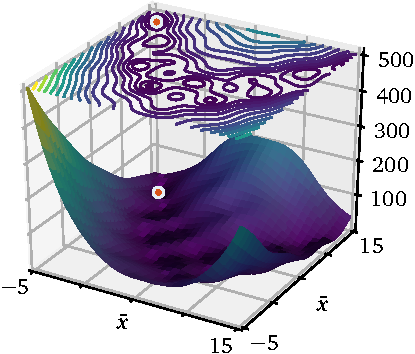
\includegraphics{optimizationProblem_1}%
  }%
  \hfill%
  \subcaptionbox{%
    GoP%
  }[76mm]{%
    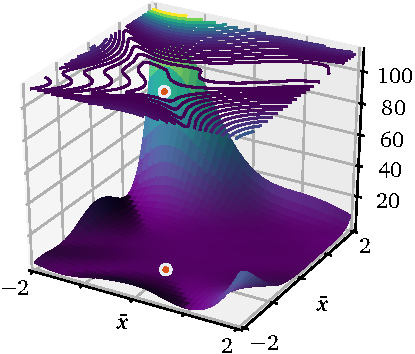
\includegraphics{optimizationProblem_2}%
  }\\[2.5mm]%
  \subcaptionbox{%
    Sch06%
  }[71mm]{%
    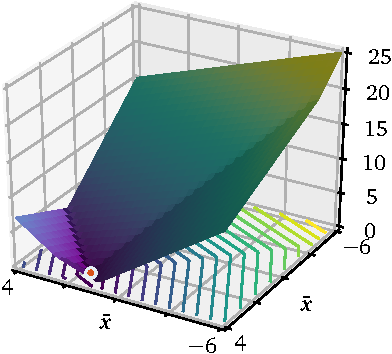
\includegraphics{optimizationProblem_3}%
  }%
  \hfill%
  \subcaptionbox{%
    Ack for $d = 2$%
  }[76mm]{%
    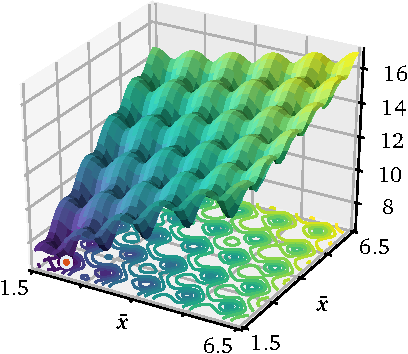
\includegraphics{optimizationProblem_4}%
  }\\[2.5mm]%
  \subcaptionbox{%
    Alp02 for $d = 2$%
  }[71mm]{%
    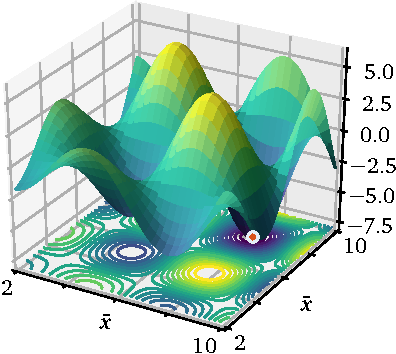
\includegraphics{optimizationProblem_5}%
  }%
  \hfill%
  \subcaptionbox{%
    Sch22 for $d = 2$%
  }[76mm]{%
    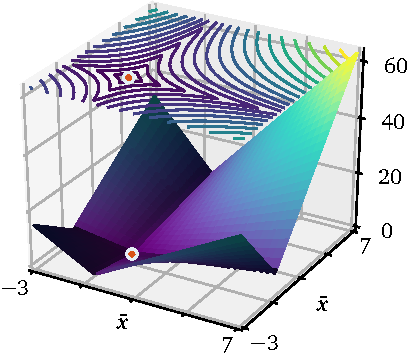
\includegraphics{optimizationProblem_6}%
  }%
  \caption[%
    Unconstrained test problems%
  ]{%
    Bivariate test functions $\objfunscaled$ in unconstrained optimization.
    The \textcolor{C1}{red dot} indicates the location of the
    global minimum.%
  }%
  \label{fig:unconstrainedOptimizationProblem}%
\end{figure}

\begin{figure}
  \subcaptionbox{%
    G08%
  }[72mm]{%
    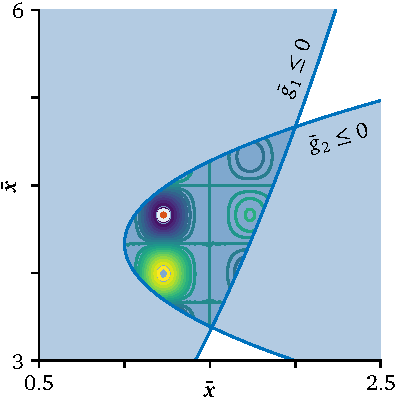
\includegraphics{optimizationProblem_7}%
  }%
  \hfill%
  \subcaptionbox{%
    G04Sq (bivariate projection over $\xscaledentry{3}$ and $\xscaledentry{5}$
    onto $\xscaledentry{t} = \xoptscaledentry{t}$ for $t = 1, 2, 4$)%
  }[72mm]{%
    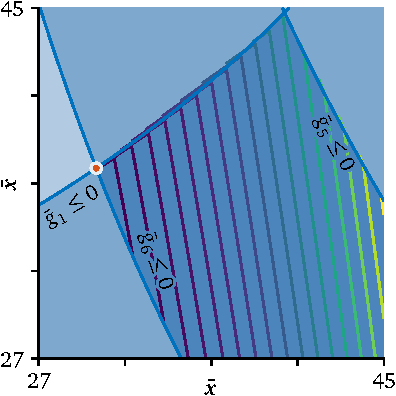
\includegraphics{optimizationProblem_8}%
  }%
  \caption[%
    Constrained test problems%
  ]{%
    Test problems in constrained optimization.
    The \textcolor{C0}{blue areas} denote the inequality constraints and
    the \textcolor{C1}{red dot} indicates the location of the
    global minimum.%
  }%
  \label{fig:constrainedOptimizationProblem}%
\end{figure}

For each test problem, we state unscaled versions of objective functions
$\objfunscaled\colon \clint{\*a, \*b} \to \real$,
$\xscaled \mapsto \objfunscaled(\xscaled)$
(and the unscaled constraint function $\ineqconfunscaled$, if present).
The actual objective function $\objfun\colon \clint{\*0, \*1} \to \real$
can be obtained by $\objfun(\*x) \ceq \objfunscaled(\xscaled)$
with the affine parameter transformation
$x_t = \tfrac{\xscaledentry{t} - a_t}{b_t - a_t}$, $t = 1, \dotsc, d$
(similarly for the constraint function).

\vspace*{1em}

The parameter domains of some test problems have been slightly translated
compared to the literature
to avoid that the minima are located exactly at or close to
the center of the domain.
In these cases, sparse grids would be in advantage as
they tend to place more points near the center of the domain
(especially for high dimensionalities).

\fillsectionornament
\section{Numerical Results}
\label{sec:54results}

\minitoc{85mm}{5}

\noindent
The following numerical experiments can be roughly divided into two parts.
First, we study interpolation errors for the test functions
to assess the effects of the hierarchical B-spline bases introduced in
\cref{chap:20sparseGrids,chap:30BSplines} on interpolation.
Second, we consider the optimality gaps $\objfun(\xoptappr) - \objfun(\xopt)$
of the calculated approximations $\xoptappr$
of the point $\xopt$ at which the objective function $\objfun$
is minimal.

\pagebreak

The results have been computed with the sparse grid toolbox \sgpp
\cite{Pflueger10Spatially},%
\footnote{%
  \url{http://sgpp.sparsegrids.org/}%
}
which has been extended in the scope of this thesis.
The new code has been written in such a way that
it is scalable and efficient, while still being maintainable and
portable \cite{Pflueger16Scalability}.



\subsection{Interpolation Error and Decay of Surpluses}
\label{sec:541interpolation}

\paragraph{Interpolation error for different test functions}

\Cref{fig:resultsInterpolationErrorTestFunctions} shows the
relative $\Ltwo$ interpolation error
$\tfrac{\normLtwo{\objfun - \sgintp}}{\normLtwo{\objfun}}$
of sparse grid interpolants $\sgintp$ to
different objective functions $\objfun$
(approximated via Monte Carlo quadrature using
$10^4$ uniformly pseudo-random samples).
The interpolation is performed on regular sparse grids of increasing levels
using hierarchical not-a-knot B-splines $\bspl[\nak]{\*l,\*i}{p}$
of degree $p = 1, 3, 5$.
As a visual aid, the plots include gray lines that indicate different
orders of convergence.

\begin{figure}
  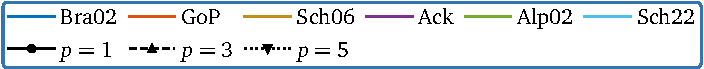
\includegraphics{resultsInterpolationLegend_1}\\[2mm]%
  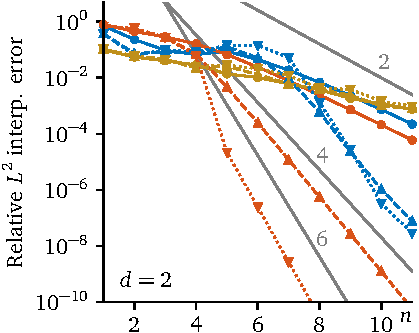
\includegraphics{resultsInterpolation_2}%
  \hfill%
  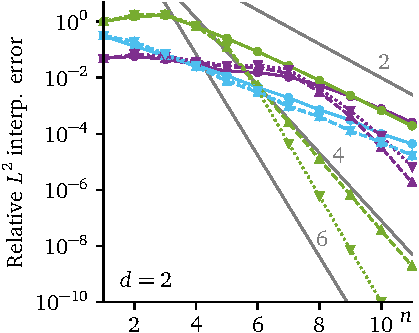
\includegraphics{resultsInterpolation_4}%
  \\[2mm]%
  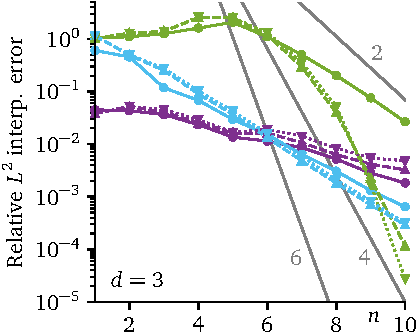
\includegraphics{resultsInterpolation_6}%
  \hfill%
  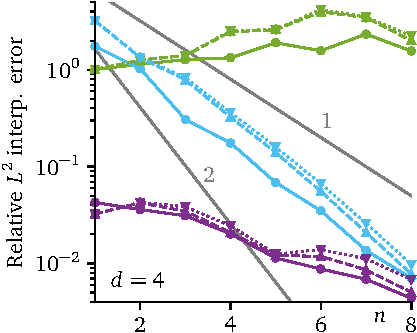
\includegraphics{resultsInterpolation_8}%
  \caption[Relative interpolation error for different test functions]{%
    Relative $\Ltwo$ interpolation error
    \vspace{-0.05em}%
    $\normLtwo{\objfun - \sgintp}/\normLtwo{\objfun}$
    for different test functions $\objfun$ \emph{(colors)}
    using hierarchical not-a-knot B-splines
    $\bspl[\nak]{\*l,\*i}{p}$ of different degrees $p$
    \emph{(line styles/markers)} on
    regular sparse grids $\regsgset{n}{d}$ of different levels $n$.%
  }%
  \label{fig:resultsInterpolationErrorTestFunctions}%
\end{figure}

It is already known that---%
if the objective function is sufficiently smooth---%
the $\Ltwo$ error of spline interpolants of degree $p$ on
$d$-dimensional regular sparse grids of level $n$
asymptotically behaves like
$\landauO{\ms{n}^{p+1} (\log_2 \ms{n}^{-1})^{d-1}}
= \landauO{2^{-(p+1)n} n^{d-1}}$ for $n \to \infty$ \cite{Sickel11Spline}.
We can numerically verify this fact easily with
\cref{fig:resultsInterpolationErrorTestFunctions},
in which we obtain the asserted orders of convergence
\pagebreak%
for the bivariate functions that are continuously differentiable.
For the functions Sch06 and Sch22, which have a non-differentiable kink,
only linear convergence can be achieved regardless of the B-spline degree.

\vspace*{\fill}

The region where the asymptotic behavior dominates largely depends
on the objective function at hand.
Functions like Bra02 and Ack with many small oscillations
require more interpolation points than ``smoother'' functions like
GoP and Alp02.
This is also the case for all functions in higher dimensionalities,
as more interpolation points are necessary to sufficiently explore the domain
(curse of dimensionality).
In \cref{fig:resultsInterpolationErrorTestFunctions}, this can already be seen
for $d \ge 3$.
This is not a consequence of employing higher-order B-splines for
the hierarchical basis.
However, it seems that higher-order B-splines lead to a slight increase
of the interpolation error in the preasymptotic range.

\pagebreak

\paragraph{Interpolation error for different basis functions}

In \cref{fig:resultsInterpolationErrorBasisFunctions},
we fix the objective function and study the influence of the choice
of hierarchical basis functions on the interpolation error.
Shown are eight types of hierarchical B-spline bases as introduced in
\cref{chap:20sparseGrids,chap:30BSplines} for the degrees $p = 1, 3, 5$.
Note that some lines exactly overlap, which is indicated in
the figure.

For $p = 1$, the non-modified bases and the modified bases coincide.
For higher degrees, the modified bases show worse results than
the corresponding non-modified versions for the same level $n$.
However, modified bases need significantly less grid points
(no boundary points),
which means that a direct comparison based on the sparse grid level $n$
is somewhat skewed.
%
In addition, we see that the not-a-knot bases coincide exactly for $p > 1$,
as they span the same space for regular and
dimensionally adaptive sparse grids.
Only with the not-a-knot boundary conditions, we obtain the true
theoretical order of convergence, which is $p + 1$ for degree $p$.
Otherwise, only quadratic convergence can be achieved regardless of $p$,
albeit with a smaller constant (offset).

\begin{SCfigure}
  \begin{minipage}{98mm}%
    \hspace*{4mm}%
    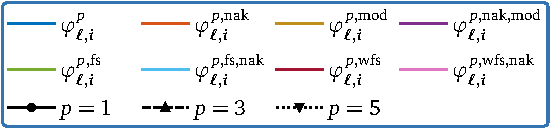
\includegraphics{resultsInterpolationLegend_2}\\[2mm]%
    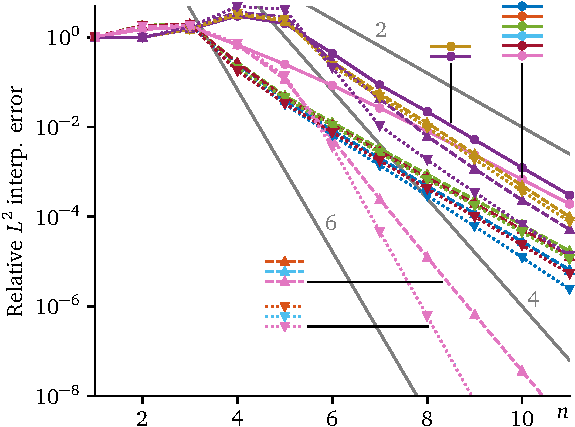
\includegraphics{resultsInterpolation_10}%
  \end{minipage}%
  \caption[Relative interpolation error for different basis functions]{%
    Relative $\Ltwo$ interpolation error
    $\normLtwo{\objfun - \sgintp}/\normLtwo{\objfun}$
    for the bivariate Alp02 function ($d = 2$)
    using different hierarchical basis functions
    $\basis{\*l,\*i}$ \emph{(colors)}
    of different degrees $p$ \emph{(line styles/markers)} and
    regular sparse grids $\regsgset{n}{d}$ of different levels $n$.\\
    The basis functions shown here involve
    standard \emph{(no superscript),}
    not-a-knot ($\mathrm{nak}$),
    modified ($\mathrm{mod}$),
    fundamental ($\mathrm{fs}$), and
    weakly fundamental ($\mathrm{wfs}$)
    splines as well as the combinations
    introduced in \cref{chap:20sparseGrids,chap:30BSplines}.%
  }%
  \label{fig:resultsInterpolationErrorBasisFunctions}%
\end{SCfigure}

\vspace*{-0.5em}

\paragraph{Pointwise interpolation error}

The importance of not-a-knot boundary conditions is also evident
from plots of the pointwise interpolation error as in
\cref{fig:resultsInterpolationErrorPointwise}.
The interpolation error grows for the standard hierarchical
B-spline basis $\bspl{\*l,\*i}{p}$
as we move towards the boundary of the domain $\clint{\*0, \*1}$,
before dropping to zero or near-zero values at or near boundary grid points.
With not-a-knot B-splines $\bspl[\nak]{\*l,\*i}{p}$,
the interpolation error is uniformly low.
For comparison, modified B-splines $\bspl[\modified]{\*l,\*i}{p}$
incur even worse issues near the boundary, since the corresponding sparse grids
do not contain boundary points.

\begin{figure}
  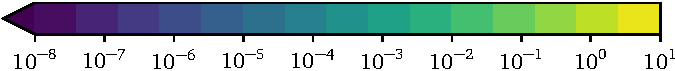
\includegraphics{resultsInterpolationPointwise_4}\\[2mm]%
  \subcaptionbox{%
    $\bspl{\*l,\*i}{p}\vphantom{\bspl[\nak]{\*l,\*i}{p}}$%
  }[48mm]{%
    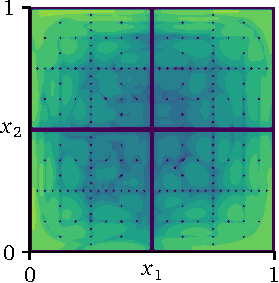
\includegraphics{resultsInterpolationPointwise_1}%
  }%
  \hfill%
  \subcaptionbox{%
    $\bspl[\nak]{\*l,\*i}{p}$%
  }[48mm]{%
    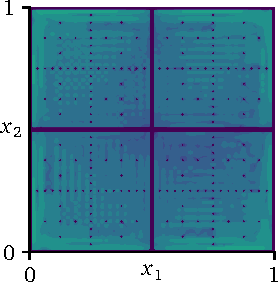
\includegraphics{resultsInterpolationPointwise_2}%
  }%
  \hfill%
  \subcaptionbox{%
    $\bspl[\modified]{\*l,\*i}{p}$%
  }[48mm]{%
    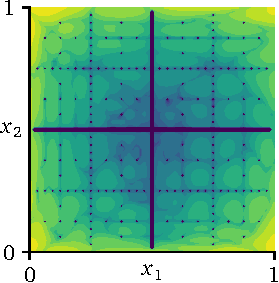
\includegraphics{resultsInterpolationPointwise_3}%
  }%
  \caption[Pointwise interpolation error for the GoP function]{%
    Pointwise interpolation error
    $\abs{\objfun(\*x) - \sgintp(\*x)}$ on a logarithmic scale
    for the bivariate GoP function ($d = 2$)
    using different hierarchical basis functions
    $\basis{\*l,\*i}$ \emph{(left, center, right)} of degree $p = 3$ on
    the regular sparse grid $\regsgset{n}{d}$ of level $n = 7$.%
  }%
  \label{fig:resultsInterpolationErrorPointwise}%
\end{figure}

\vspace*{-0.3em}

\paragraph{Decay of surpluses}

In the piecewise linear case ($p = 1$),
the hierarchical surpluses $\surplus{\*l,\*i}$
can be represented as the $\Ltwo$ inner product of
the corresponding hat function $\bspl{\*l,\*i}{1}$ with the
second mixed derivative
$\partialderiv[2d]{\partialdiff x_1^2 \dotsm \partialdiff x_d^2}{\objfun}$
of the objective function $\objfun$,
if $\*l \ge \*1$ and if this derivative exists and is continuous
(see \cref{eq:surplusIntegral}).
Consequently, one can prove that
$\abs{\surplus{\*l,\*i}} \le 2^{-d} 2^{-2\normone{\*l}}
\normLinftyscaled{
  \partialderiv[2d]{\partialdiff x_1^2 \dotsm \partialdiff x_d^2}{\objfun}
}$ \cite{Bungartz04Sparse},
i.e., the absolute values of the hierarchical surpluses
decay  in quadratic order with the level sum $\normone{\*l}$.
This relation can be used to estimate the convergent range
of the corresponding interpolation error (\cref{%
  fig:resultsInterpolationErrorTestFunctions,%
  fig:resultsInterpolationErrorBasisFunctions%
}).
A generalization of this estimate to higher B-spline degrees $p > 1$
is not straightforward, as the surpluses $\surplus{\*l,\*i}$
then also depend on function values $\objfun(\gp{\*l',\*i'})$ at
grid points of higher levels $\*l' \ge \*l$.

The decay of surpluses can be seen in \cref{fig:resultsDecaySurpluses},
which shows the mean absolute value of surpluses corresponding to
grid points grouped by their level sum $\normone{\*l}$.
Due to the dependency of coarse-level surpluses on high-level grid points
for $p > 1$,
we have to fix the level $n$ of the regular sparse grid for this analysis.
\Cref{fig:resultsDecaySurpluses} suggests that the
absolute value of the surpluses decays with order $p + 1$ for
B-spline degree $p$, although no theoretical evidence
is known to support this claim.
Higher B-spline degrees seem to imply that
$\abs{\surplus{\*l,\*i}}$ generally increases, if $\normone{\*l}$ is
in the preasymptotic range.

\begin{figure}
  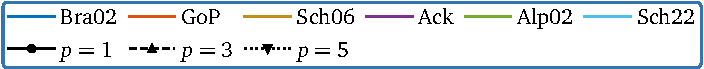
\includegraphics{resultsInterpolationLegend_1}\\[2mm]%
  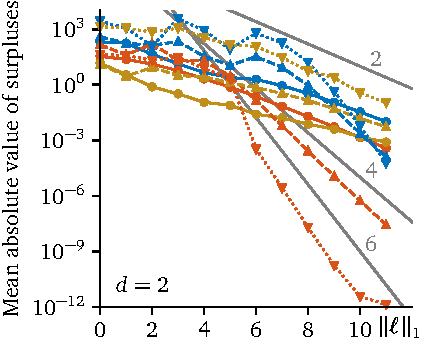
\includegraphics{resultsInterpolation_1}%
  \hfill%
  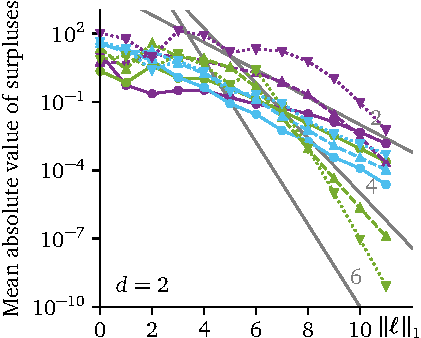
\includegraphics{resultsInterpolation_3}%
  \caption[Decay of surpluses for different test functions]{%
    Mean absolute value of surpluses by level sum $\normone{\*l}$
    \vspace{-0.05em}%
    for different test functions $\objfun$ \emph{(colors)}
    using hierarchical not-a-knot B-splines
    $\bspl[\nak]{\*l,\*i}{p}$ of different degrees $p$
    \emph{(line styles/markers)} on
    the regular sparse grid $\regsgset{n}{d}$ of level $n = 11$.%
  }%
  \label{fig:resultsDecaySurpluses}%
\end{figure}



\subsection{Complexity of Hierarchization}
\label{sec:543complexity}

In \cref{chap:40algorithms}, we introduced a number of new
hierarchical spline bases with the aim to reduce the complexity
of algorithms with the key example of hierarchization.
In the following, we study the suitability of the new bases
to achieve this goal \cite{Valentin18Fundamental}.

\paragraph{Complexity of fundamental splines}

\Cref{fig:complexityFundamental} compares the hierarchization complexity of
modified hierarchical B-splines $\bspl[\modified]{\*l,\*i}{p}$ with the new
modified hierarchical fundamental splines $\bspl[\fs,\modified]{\*l,\*i}{p}$
as measured on a laptop with Intel Core i5-4300U.
For the modified hierarchical B-spline basis,
we solve a linear system of size $\ngp \times \ngp$,
for which Gaussian elimination takes
$\landauTheta{\ngp^3}$ time and $\landauTheta{\ngp^2}$ memory for
$\ngp \to \infty$ (where $\ngp$ is the number of sparse grid points and
$d$ is assumed to be constant).
More sophisticated methods to solve linear systems
are not able to significantly
reduce this complexity without any further assumptions on the system matrix
$\intpmat$ (e.g., symmetry, positive definiteness, or bandedness).
As $\ngp$ grows,
the space needed to store an $\ngp \times \ngp$ matrix quickly exceeds
the available memory.

For the modified hierarchical fundamental splines,
we can use the \bfs algorithm presented in \cref{sec:44spatAdaptiveBFS}.
\bfs works in quadratic time $\landauO{\ngp^2}$, but more importantly,
it works in linear space $\landauO{\ngp}$.
Both can be seen very well in \cref{fig:complexityFundamental}:
The computation time drops from cubic to quadratic complexity for fundamental splines
and the consumed memory is reduced from quadratic to linear complexity.

\begin{figure}
  
\includegraphics{complexityFundamental_3}\\[2mm]%
  \subcaptionbox{%
    Computation time%
  }[72mm]{%
    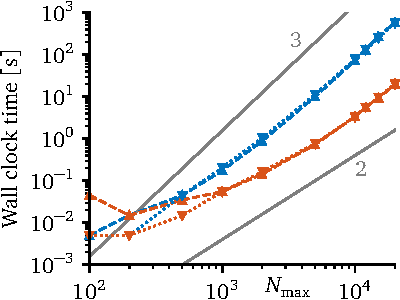
\includegraphics{complexityFundamental_1}%
  }%
  \hfill%
  \subcaptionbox{%
    Memory consumption%
  }[72mm]{%
    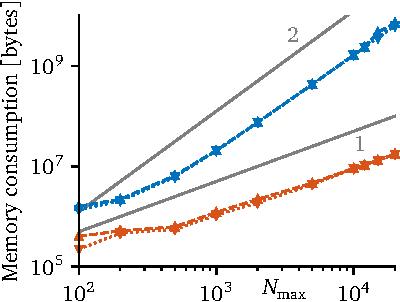
\includegraphics{complexityFundamental_2}%
  }%
  \caption[Complexity of fundamental splines]{%
    Computation time and memory consumption of hierarchization
    with modified hierarchical B-splines
    $\bspl[\modified]{\*l,\*i}{p}$ \emph{\textcolor{C0}{(blue)}} and
    \vspace*{-0.3em}%
    modified hierarchical fundamental splines
    $\bspl[\fs,\modified]{\*l,\*i}{p}$ \emph{\textcolor{C1}{(red)}}
    of degrees $p = 3$ and $p = 5$
    on the spatially adaptive sparse grids generated by the criterion of
    Novak--Ritter for the optimization of Ack with $d = 4$ and
    $\ngpMax$ grid points.
    Adapted from \cite{Valentin18Fundamental}.%
  }%
  \label{fig:complexityFundamental}%
\end{figure}

\paragraph{Complexity of weakly fundamental splines}

It is not straightforward to include weakly fundamental splines
in \cref{fig:complexityFundamental} as we have to insert missing
chain points to apply the unidirectional principle
(see \cref{sec:45spatAdaptiveUP}).
As this increases the number of necessary evaluations of $\objfun$,
a comparison of computation times with standard B-splines would be skewed.
Instead, we study in \cref{fig:complexityWeaklyFundamental}
the number of grid points that have to be inserted
to ensure the correctness of the unidirectional principle.
As we have seen in \cref{sec:453chains}
(cf.\ \cref{fig:chainInsertionBSpline}),
inserting all chains needed for standard hierarchical B-splines
often results in a full grid, which suffers from the curse of dimensionality.
%
\begin{figure}
  
\includegraphics{complexityWeaklyFundamental_4}\\[2mm]%
  \subcaptionbox{%
    $\gamma = 0.05$%
  }[48mm]{%
    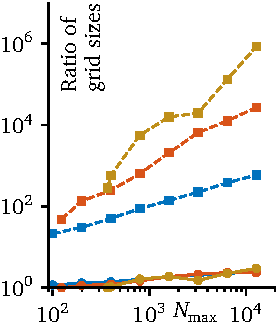
\includegraphics{complexityWeaklyFundamental_1}%
  }%
  \hfill%
  \subcaptionbox{%
    $\gamma = 0.15$%
  }[48mm]{%
    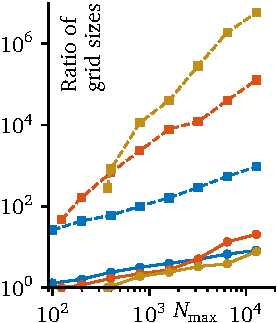
\includegraphics{complexityWeaklyFundamental_2}%
  }%
  \hfill%
  \subcaptionbox{%
    $\gamma = 0.25$%
  }[48mm]{%
    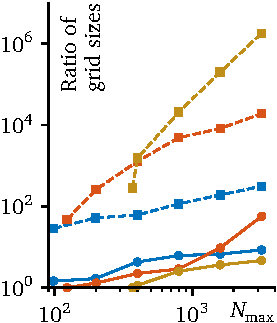
\includegraphics{complexityWeaklyFundamental_3}%
  }%
  \caption[Complexity of weakly fundamental splines]{%
    Total number of grid points after inserting all missing chains
    for cubic weakly fundamental not-a-knot splines
    $\bspl[\wfs,\nak]{\*l,\*i}{p}$ \emph{($p = 3$, solid lines),}
    and after inserting all missing full grid points \emph{(dashed).}
    Shown are the ratios of the resulting grid sizes to the
    initial grid sizes before inserting points.
    The initial grids are the spatially adaptive sparse grids generated
    by the criterion of Novak--Ritter for the optimization of Ack with
    different dimensionalities \emph{(colors)},
    different adaptivity parameters $\gamma$ \emph{(left, center, right),}
    and $\ngpMax$ grid points.%
  }%
  \label{fig:complexityWeaklyFundamental}%
\end{figure}%
%
This can be seen in \cref{fig:complexityWeaklyFundamental}
for hierarchical not-a-knot B-splines (dashed lines).
By inserting all full grid points,
the number of grid points increases by several orders of magnitude:
If the initial grid has $\ngpMax = \num{10000}$ points,
then the grid size increases roughly by the factor $10^2$ for $d = 2$,
$10^4$ for $d = 3$, and $10^6$ for $d = 4$,
resulting in computationally infeasible
grids with $10^6$, $10^8$, and $10^{10}$ points, respectively.
If we instead only insert the missing chain points needed for the
hierarchical weakly fundamental not-a-knot basis
(solid lines, cf.\ \cref{fig:chainInsertionWeaklyFundamentalSpline}),
then the number of grid points increases only slightly.
For grids that have a low adaptivity (which correspond
to low adaptivity parameters $\gamma$ in the Novak--Ritter criterion,
see \cref{sec:521novakRitter}), the grid size only increases by the
factor of two.
For highly-adaptive grids
(corresponding to large $\gamma$),
the number of necessary chain grid points increases significantly.



\subsection{Optimality Gap}
\label{sec:542optimization}

\paragraph{Optimality gaps and displacements}

With the method described in \cref{sec:52method},
we find approximations $\xoptappr$ of the
global minimum $\xopt$ of some objective function $\objfun$
using optimization of a B-spline surrogate $\sgintp$ of $\objfun$
on sparse grids.
Obviously, the more accurate the sparse grid surrogate is,
the better the approximation $\xoptappr$ will be.
In the following plots,
we show the optimality gaps $\objfun(\xoptappr) - \objfun(\xopt)$
in terms of function values.%
\footnote{%
  In order to calculate the optimality gap,
  it is crucial to determine $\objfun(\xopt)$ as exact as possible.
  Otherwise, the optimality gap might either not converge to zero
  or it might even become negative.%
}
The results are sensitive to even small displacements
of the objective function, i.e.,
the results may change for the
function $\*x \mapsto \objfun(\*x - \*a)$
instead of $\*x \mapsto \objfun(\*x)$ for $\*x \in \clint{\*0, \*1}$
and some small $\*a \in \real^d$.%
\footnote{%
  By using the formulas in \cref{chap:a20testProblems},
  all test functions $\objfun$ in \cref{sec:53testProblems}
  can be extended such that they can be evaluated at $\*x - \*a$
  for all $\*x \in \clint{\*0, \*1}$, if $\*a \in \real^d$ is small enough.
  Note that we set $a_t$ to zero if a non-zero displacement in
  the $t$-th component would change the location of the global minimum.%
}
Therefore, the optimization for each of the
data points for \cref{%
  fig:resultsOptimizationUnconstrainedTestFunctions,%
  fig:resultsOptimizationConstrainedTestFunctions%
}
was repeated five times with replacements $\*a$
whose entries $a_t$ were independent and identically distributed Gaussian
pseudo-random numbers with zero mean and a standard deviation of $0.01$.
The optimality gaps shown in the figures of this section were computed
as the mean of the five runs to increase confidence in the results.

\paragraph{Unconstrained optimization}

\Cref{fig:resultsOptimizationUnconstrainedTestFunctions}
shows the optimality gaps for different test functions $\objfun$
over the number $\ngpMax$ of allowed evaluations of $\objfun$.
For the continuously differentiable functions
Bra02, GoP\punctfix{,} Ack, and Alp02
in $d = 2$ dimensions (top row),
the optimization of the corresponding cubic B-spline surrogates (solid lines)
performs significantly better than using piecewise linear basis functions
(dashed lines).
The reason is two-fold:
First, by using higher-order basis functions, the surrogates are more accurate
in general as seen in the discussion of the interpolation error in
\cref{sec:541interpolation}.
Second, the availability of surrogate gradients accelerates the
convergence of the employed optimization methods.
For some test functions, B-splines give better results than even
the direct optimization of the objective function (dotted lines).

\begin{figure}
  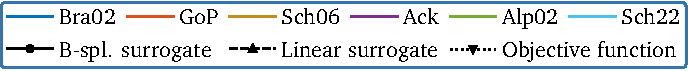
\includegraphics{resultsOptimizationLegend_1}\\[2mm]%
  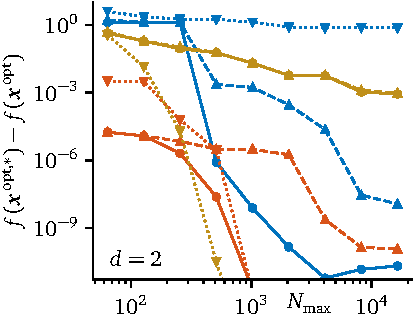
\includegraphics{resultsOptimizationUnconstrained_1}%
  \hfill%
  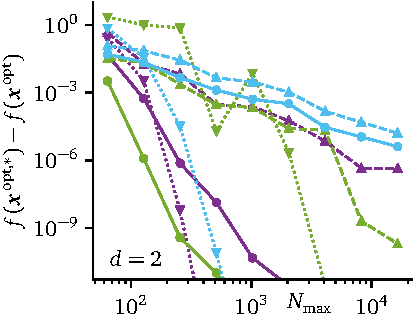
\includegraphics{resultsOptimizationUnconstrained_2}%
  \\[2mm]%
  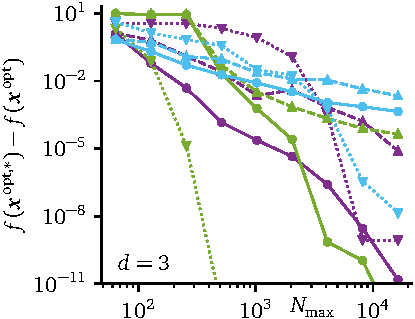
\includegraphics{resultsOptimizationUnconstrained_3}%
  \hfill%
  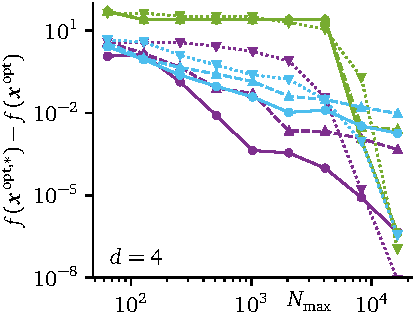
\includegraphics{resultsOptimizationUnconstrained_4}%
  \\[2mm]%
  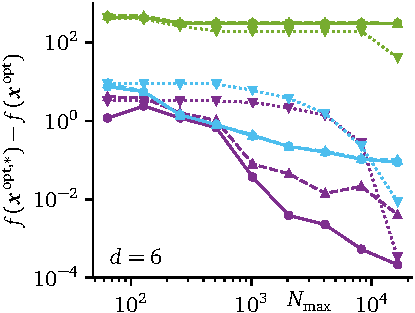
\includegraphics{resultsOptimizationUnconstrained_5}%
  \hfill%
  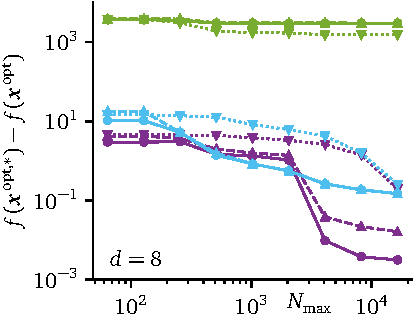
\includegraphics{resultsOptimizationUnconstrained_6}%
  \caption[Optimality gaps for different objective functions (unconstrained)]{%
    Optimality gaps $\objfun(\xoptappr) - \objfun(\xopt)$ between
    the function value at the approximated optimum $\xoptappr$ and
    the minimal function value at the actual optimum $\xopt$
    over the number $\ngpMax$ of objective function evaluations
    for different unconstrained
    objective functions $\objfun$ \emph{(colors).}
    Shown are the optimization results of the B-spline surrogate
    \emph{(solid lines),}
    the optimization results of the piecewise linear surrogate
    \emph{(dashed),} and
    the optimization results of the actual objective function
    \emph{(dotted)} as described in \cref{sec:52method}.%
  }%
  \label{fig:resultsOptimizationUnconstrainedTestFunctions}%
\end{figure}

For the test functions Sch06 and Sch22 with discontinuous derivatives,
the advantage of higher-order B-splines is not as evident (Sch22) or
does not even exist (Sch06).
However, in low dimensions, i.e., $d \le 4$, B-splines
achieve a slight advantage compared to the piecewise linear basis
for the Sch22 function.
In higher dimensionalities, i.e., $d \ge 6$ (bottom row),
convergence visibly slows down for all methods shown in
\cref{fig:resultsOptimizationUnconstrainedTestFunctions},
although for some objective functions, B-splines are still able
to perform better than the comparison methods
(most notably for the Ack function).

\paragraph{Constrained optimization}

\Cref{fig:resultsOptimizationConstrainedTestFunctions}
shows the result for the two constrained optimization problems.
The objective function value $\objfun(\xoptappr)$
at the approximated optimum $\xoptappr$ should not only
be as small as possible, but $\xoptappr$ should also be feasible, i.e.,
$\ineqconfun(\xoptappr) \le \*0$.
Hence, we also plot the maximal violation
$\norm[\infty]{\nonnegpart{\ineqconfun(\xoptappr)}}$
of the constraints in the respective optimal points $\xoptappr$.

\begin{figure}
  
\includegraphics{resultsOptimizationLegend_2}\\[2mm]%
  \subcaptionbox{%
    G08%
  }[72mm]{%
    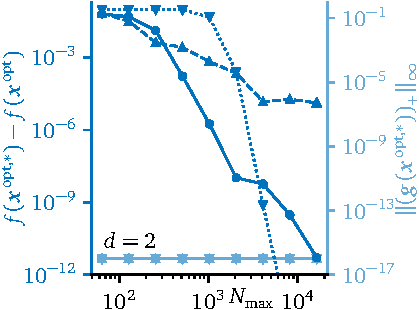
\includegraphics{resultsOptimizationConstrained_1}%
  }%
  \hfill%
  \subcaptionbox{%
    G04Sq%
  }[72mm]{%
    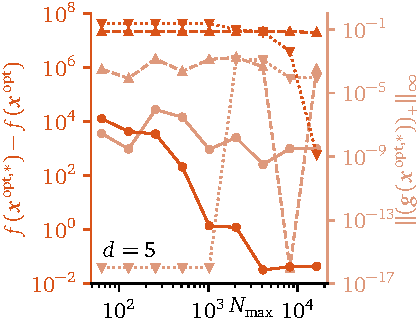
\includegraphics{resultsOptimizationConstrained_2}%
  }%
  \caption[Optimality gaps for different objective functions (constrained)]{%
    Optimality gaps $\objfun(\xoptappr) - \objfun(\xopt)$ between
    the function value at the approximated optimum $\xoptappr$ and
    the minimal function value at the actual optimum $\xopt$
    over the number $\ngpMax$ of objective function evaluations
    for different constrained optimization problems
    \emph{(dark, left vertical axes).}
    In addition to the lines of
    \cref{fig:resultsOptimizationUnconstrainedTestFunctions},
    the constraint violation
    $\norm[\infty]{\nonnegpart{\ineqconfun(\xoptappr)}}$
    at the approximated optimum $\xoptappr$ is plotted
    \emph{(light, right vertical axes).}%
  }%
  \label{fig:resultsOptimizationConstrainedTestFunctions}%
\end{figure}

For the bivariate G08 problem, the hierarchical B-splines surrogates
perform better than the direct gradient-free optimization of the problem
for $\ngpMax \le 3500$ objective function evaluations
and better than the piecewise linear surrogate for $\ngpMax \ge 300$
objective function evaluations.
All calculated points are feasible.%
\footnote{%
  For plotting reasons,
  \cref{fig:resultsOptimizationConstrainedTestFunctions} shows
  $\max(\norm[\infty]{\nonnegpart{\ineqconfun(\xoptappr)}}, 10^{-16})$
  instead of the true constraint violation.%
}

The range of the objective function of the five-dimensional G04Sq problem
is larger than the range of G08.
This results in generally higher optimality gaps
$\objfun(\xoptappr) - \objfun(\xopt)$ as we do not normalize
with respect to the range.
B-splines achieve good approximations $\xoptappr$
of $\xopt$ already for $\ngpMax = 1000$ with an optimality gap of
around one.
Both comparison methods show optimality gaps that are
seven orders of magnitude higher.

Additionally, the corresponding values of constraint violation
are between $10^{-10}$ and $10^{-6}$, i.e.,
the constraints are numerically met.
In contrast, the optimizers struggle more for
the comparison methods (optimization of the linear surrogate and
of the objective function) to meet the constraints,
as the values of the constraint violation partly exceed $10^{-3}$.
The availability of gradients seems to allow the constrained optimization
methods to better enforce the feasibility of the
resulting points $\xoptappr$.

Note that while the results look already promising for the B-spline surrogate
method, these results could still be improved upon.
The Novak--Ritter criterion used to generate the
spatially adaptive sparse grids does not take the constraints into account.
Consequently, many sparse grid points are created outside the feasible domain.
By modifying the criterion to prefer points that are in a neighborhood of
the feasible domain, the quality of the interpolant
close to potential optima should increase.

\section{Example Application: Fuzzy Extension Principle}
\label{sec:55fuzzy}

\minitoc[-1mm]{84mm}{4}

\noindent
To conclude this chapter, we consider the fuzzy extension principle
as an example application of optimization of B-spline sparse grid surrogates.

\paragraph{Aleatoric and epistemic uncertainties}

Classical uncertainty quantification (UQ) distinguishes between
aleatoric and epistemic uncertainties \cite{Walz16Fuzzy}.
Aleatoric uncertainties result from the variability of inputs or
model components and from the ``intrinsic randomness''
of quantities.
They are best described by probability theory, giving exact probabilities.
Epistemic uncertainties arise from subjectivity,
simplifying modeling assumptions, and incomplete knowledge.
These uncertainties are better captured by fuzzy theory,
which is more imprecise than the ``exact'' stochastic assumptions
of probabilities \cite{Walz16Fuzzy}.

\paragraph{Uncertainty quantification with fuzzy uncertainties}

In uncertainty quantification, the key question is as follows:
Given a model and uncertain input parameters for the model,
how uncertain is the model output?
While there are many approaches available
for probabilistic uncertainties,
it is not straightforward to solve this task
for fuzzy uncertainties.
Fortunately, Zadeh proposed in 1975
the \term{fuzzy extension principle} \cite{Zadeh75Concept},
which addresses this very question.

\paragraph{Sparse grids and B-splines for fuzzy uncertainties}

As we explain in this section,
the fuzzy extension principle requires the solution of numerous
optimization problems that involve the original objective function
$\objfun$.
This predestines the replacement of $\objfun$ with sparse grid surrogates,
as explained in the beginning of the chapter.
Previous work by Klimke \cite{Klimke06Uncertainty} already
studied this approach for piecewise linear functions on uniform sparse grids
and for global polynomials on sparse Clenshaw--Curtis grids.
We assess the suitability of interpolation with higher-order
hierarchical B-splines on sparse grids for the fuzzy extension principle.
It should be mentioned that there is also work
directly incorporating (non-hierarchical) B-splines
into the framework of fuzzy theory for modeling uncertain surfaces
\multicite{Anile00Modeling,Zakaria14Fuzzy}.



\subsection{Fuzzy Sets and Fuzzy Intervals}
\label{sec:551fuzzySets}

In the following, we repeat very briefly the necessary
definitions of basic fuzzy theory.
Examples for the definitions are shown in \cref{fig:fuzzySet}.
A more in-depth introduction can be found in
\multicite{Hanss05Applied,Klimke06Uncertainty,Walz16Fuzzy}.

\begin{figure}
  \subcaptionbox{%
    Non-convex fuzzy set \emph{\textcolor{C0}{(blue)}}
    and $\alpha$-cut \emph{\textcolor{C1}{(red)}.}%
  }[46mm]{%
    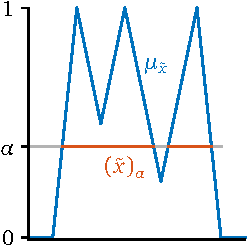
\includegraphics{fuzzySet_1}%
  }%
  \hfill%
  \subcaptionbox{%
    Fuzzy interval.%
  }[43mm]{%
    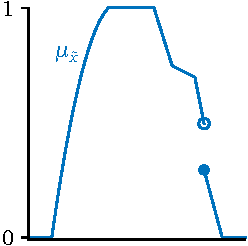
\includegraphics{fuzzySet_2}%
  }%
  \hfill%
  \subcaptionbox{%
    Common types of fuzzy numbers and intervals (see text).%
  }[56mm]{%
    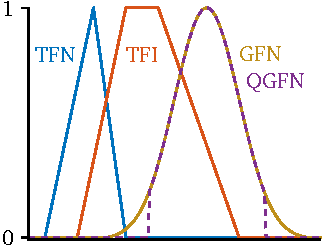
\includegraphics{fuzzySet_3}%
  }%
  \caption[%
    Examples of fuzzy sets and $\alpha$-cuts%
  ]{%
    Examples of membership functions of fuzzy sets and $\alpha$-cuts.%
  }%
  \label{fig:fuzzySet}%
\end{figure}

\paragraph{Fuzzy sets}

Let $X \subset \real$ be a closed interval on the real line
and $\memfun{x}\colon X \to \clint{0, 1}$ be a function.
We call the graph $\fuzzy{x} \ceq \{(x, \memfun{x}(x) \mid x \in X\}$
of $\memfun{x}$ a \term{fuzzy set} with
\term{membership function} $\memfun{x}$.
Fuzzy sets generalize ordinary subsets of $X$,
which can be obtained by requiring $\memfun{x}(X) \subset \{0, 1\}$.
In this case, the fuzzy set is called \term{crisp} and
$\fuzzy{x}$ can be identified with the ordinary set
$\{x \in X \mid \memfun{x}(x) = 1\}$.
A fuzzy set $\fuzzy{x}$ is \term{normalized}
if $\max_{x \in X} \memfun{x}(x) = 1$.
A \term{convex} fuzzy set $\fuzzy{x}$ satisfies
$\min(\memfun{x}(a), \memfun{x}(c)) \le \memfun{x}(b)$ for all $a, b, c \in X$
with $a \le b \le c$.

\paragraph{Fuzzy intervals and $\alpha$-cuts}

A convex and normalized fuzzy set $\fuzzy{x}$ with
piecewise continuous membership function $\memfun{x}$ is called
\term{fuzzy interval.}
If $\{x \in X \mid \memfun{x}(x) = 1\} = \{a\}$ for some $a \in X$,
then the fuzzy interval $\fuzzy{x}$ is called \term{fuzzy number.}

For $\alpha \in \clint{0, 1}$, the $\alpha$-cut of $\fuzzy{x}$ is
defined as $\acut{x}{\alpha} \ceq \{x \in X \mid \memfun{x}(x) \ge \alpha\}$
for $\alpha > 0$ and $\acut{x}{0} \ceq \supp \memfun{x}$ for $\alpha = 0$.
The $\alpha$-cuts of fuzzy intervals $\fuzzy{x}$ are always
nested closed intervals, i.e.,
$\acut{x}{\alpha} = [a, b]$ for some $a \le b$ and
$\acut{x}{\alpha_1} \supset \acut{x}{\alpha_2}$ for $\alpha_1 \le \alpha_2$.

\paragraph{Common types of fuzzy numbers and intervals}

There are various types of fuzzy numbers and intervals
\cite{Klimke06Uncertainty}.
Most common are
\term{triangular fuzzy numbers} (TFNs, i.e., linear B-splines),
\term{trapezoidal fuzzy intervals}
(TFIs, where a plateau of height one is inserted at the peak, i.e.,
sums of two neighboring linear B-splines), and
\term{Gaussian fuzzy numbers} (GFNs) with membership function
$\memfun{x}(x) = \exp(-\frac{(x - \mu)^2}{(2\sigma)^2})$.
As the support of Gaussian fuzzy numbers is unbounded,
\term{quasi-Gaussian fuzzy numbers} (QGFNs) truncate the support
to a fixed multiple of the standard deviation $\sigma$
\cite{Klimke06Uncertainty}.
However, it would be more natural to directly employ B-splines of
degree $p > 1$ (normalized adequately), since they generalize
triangular fuzzy numbers and their limit with respect to $p$
is a Gaussian fuzzy number.



\subsection{Fuzzy Extension Principle}
\label{sec:552fuzzyExtensionPrinciple}

Let $\objfun\colon \clint{\*0, \*1} \to \real$ be an objective function,
whose values $y = \objfun(\*x)$ represent the results of the
simulation of a model with input parameters $(x_1, \dotsc, x_d) = \*x$.
If the input parameters are uncertain and
given as fuzzy sets $\fuzzy{x}_1, \dotsc, \fuzzy{x}_d$,
what is the resulting uncertain outcome
``$\fuzzy{y} \ceq \objfun(\fuzzy{x}_1, \dotsc, \fuzzy{x}_d)$''?
Note that there is no definite answer to this question,
as ``$\objfun(\fuzzy{x}_1, \dotsc, \fuzzy{x}_d)$'' is not well-defined.
The fuzzy extension principle, suggested by Zadeh \cite{Zadeh75Concept},
provides one possible definition.

\paragraph{Alternative fuzzy extension principle}

We use an alternative formulation of the fuzzy extension principle,
which is stated in \cite{Klimke06Uncertainty}.
The original formulation is computationally more complex,
as it requires the solution of equality-constrained optimization problems
and one needs to know the range of $\objfun$, which might not be given.
The two formulations are equivalent,
if $\fuzzy{x}_1, \dotsc, \fuzzy{x}_d$ are (compactly supported)
fuzzy intervals and $\objfun$ is continuous \cite{Buckley90Using},
which we assume in the following.

The alternative fuzzy extension principle defines
``$\fuzzy{y} = \objfun(\fuzzy{x}_1, \dotsc, \fuzzy{x}_d)$'' as the fuzzy set
$\fuzzy{y}$ with
\begin{subequations}
  \label{eq:alternativeFuzzyExtensionPrinciple}
  \begin{alignat}{2}
    \memfun{y}(y)
    &\ceq \sup\{\alpha \in \clint{0, 1} \mid y \in \acut{y}{\alpha}\},\quad
    &&y \in \real,\\
    \acut{y}{\alpha}
    &\ceq \bracket*{
      \min_{\*x \in \Omega_\alpha} \objfun(\*x),\;
      \max_{\*x \in \Omega_\alpha} \objfun(\*x)
    },\quad
    &&\alpha \in \clint{0, 1},\\
    \Omega_\alpha
    &\ceq \acut[1]{x}{\alpha} \times \dotsb \times \acut[d]{x}{\alpha},\quad
    &&\alpha \in \clint{0, 1}.
  \end{alignat}
\end{subequations}
This definition is visualized in \cref{fig:fuzzyExtensionPrinciple}.
The first equation defines $\fuzzy{y}$ via its $\alpha$-cuts,
which are given in the second equation as the closed interval
between the minimal and the maximal value of $\objfun$ on some
hyper-rectangular domain $\Omega_\alpha$.
The third equation specifies this domain $\Omega_\alpha$ as the
Cartesian product of the univariate $\alpha$-cuts.
Hence, we only have to solve box-constrained optimization problems,
as opposed to the general equality-constrained problems
in the original formulation of the fuzzy extension principle.

\begin{figure}
  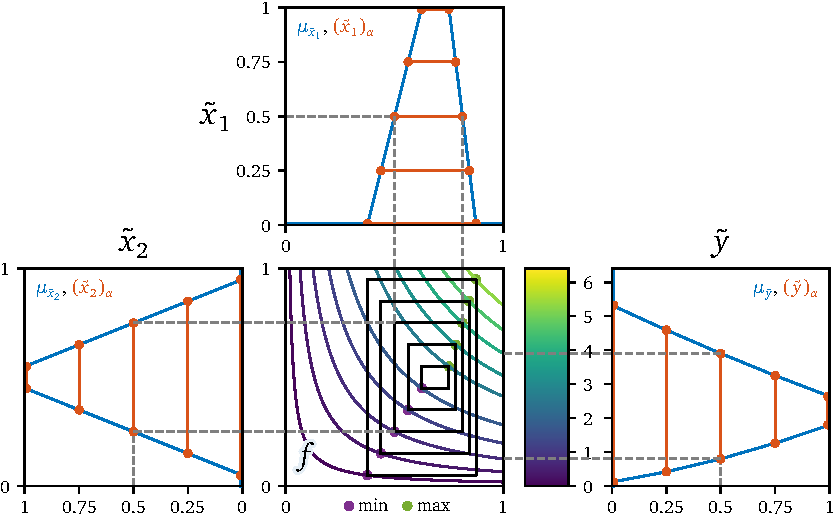
\includegraphics{fuzzyExtensionPrinciple_1}%
  \caption[%
    Alternative fuzzy extension principle%
  ]{%
    Example of the application of the
    alternative fuzzy extension principle to the bivariate objective function
    $\objfun(\*x) = 6.4 x_1 x_2$ \emph{(bottom)}
    and triangular fuzzy input intervals
    $\fuzzy{x}_1$ and $\fuzzy{x}_2$ \emph{(top and left)}
    to obtain the fuzzy output interval $\fuzzy{y}$ \emph{(right).}
    Adapted from \cite{Klimke06Uncertainty}.%
  }%
  \label{fig:fuzzyExtensionPrinciple}%
\end{figure}

\paragraph{Implementation}

The implementation of the alternative fuzzy extension principle
is straightforward and shown in \cref{alg:alternativeFuzzyExtensionPrinciple}
\cite{Klimke06Uncertainty}.
The range $\clint{0, 1}$ of $\alpha$
is discretized into $m + 1$ uniformly spaced values $\alpha_j$
(where $m \in \nat$).
For each of these values $\alpha_j$, we compute the corresponding
$\alpha_j$-cut of $\fuzzy{y}$ by solving the two box-constrained
optimization problems of \cref{eq:alternativeFuzzyExtensionPrinciple}.
The fuzzy output interval $\fuzzy{y}$ can then be approximated by
interpolating the interval bounds of the $\alpha_j$-cuts of $\fuzzy{y}$.

\begin{algorithm}
  \begin{algorithmic}[1]
    \Function{$\fuzzy{y} = \texttt{alternativeFuzzyExtensionPrinciple}$}{%
      $m$, $\fuzzy{x}_1$, \dots, $\fuzzy{x}_d$%
    }
      \For{$j = 0, \dotsc, m$}
        \State{$\alpha_j \gets j/m$}
        \ForOneLine{$t = 1, \dotsc, d$}{Compute $\acut[t]{x}{\alpha_j} = \clint{a_{j,t}, b_{j,t}}$}
        \State{%
          $\Omega_{\alpha_j} \gets \acut[1]{x}{\alpha_j} \times \dotsb \times
          \acut[d]{x}{\alpha_j} = \clint{\*a_j, \*b_j}$%
        }
        \State{%
          Solve $\min_{\*x \in \Omega_{\alpha_j}} \objfun(\*x)$ and
          $\max_{\*x \in \Omega_{\alpha_j}} \objfun(\*x)$%
        }
        \State{%
          $\acut{y}{\alpha_j} = [c_j, d_j] \gets \clint{
            \min_{\*x \in \Omega_{\alpha_j}} \objfun(\*x),
            \max_{\*x \in \Omega_{\alpha_j}} \objfun(\*x)
          }$
        }
      \EndFor{}\vspace{-2mm}
      \State{%
        $D \gets
        \{(c_j, \alpha_j) \mid j = 0,\, 1,\, \dotsc,\, m\} \cup
        \{(d_j, \alpha_j) \mid j = m,\, m - 1,\, \dotsc,\, 0\}$%
      }
      \State{%
        $\memfun{y} \gets \text{Piecewise linear interpolant of $D$}$%
      }%
      \Comment{extend to $X$ by zero}%
    \EndFunction{}
  \end{algorithmic}
  \caption[Alternative fuzzy extension principle]{%
    Alternative fuzzy extension principle.
    Inputs are the number of $\alpha$ segments to use as discretization and
    the $d$ fuzzy intervals $\fuzzy{x}_1, \dotsc, \fuzzy{x}_d$
    (we have to be able to determine $\alpha$-cuts
    of these fuzzy input intervals).
    The output is an approximation to the output $\fuzzy{y}$
    of the alternative fuzzy extension principle
    (given by an approximation of its membership function $\memfun{y}$).%
  }%
  \label{alg:alternativeFuzzyExtensionPrinciple}%
\end{algorithm}



\subsection{Using B-Splines on Sparse Grids to Propagate Fuzzy Uncertainties}
\label{sec:553fuzzyBSplines}

Following Klimke's approach \cite{Klimke06Uncertainty},
we replace the objective function $\objfun$ in
\cref{alg:alternativeFuzzyExtensionPrinciple}
with a sparse grid surrogate $\sgintp$.
The solution of the optimization problems
$\min_{\*x \in \Omega_{\alpha_j}} \sgintp(\*x)$ and
$\max_{\*x \in \Omega_{\alpha_j}} \sgintp(\*x)$ with respect to the
surrogate $\sgintp$ instead of the true objective function $\objfun$
takes significantly less time, if evaluations of the objective function
are expensive.

However, Klimke used piecewise linear functions as the hierarchical basis on
uniform sparse grids and global polynomials on sparse Clenshaw--Curtis grids.
The drawbacks of each of the bases are evident:
First, piecewise linear surrogates are not continuously differentiable and
can thus not be optimized well with gradient-based optimization methods.
Second, global polynomials are only suitable for
Clenshaw--Curtis grids (Chebyshev-distributed points)
due to Runge's phenomenon,
unnecessarily restricting the choice of grid points.
Hierarchical B-splines of degree $p$ are $(p - 1)$ times
continuously differentiable and defined for arbitrary point
distributions, eliminating both drawbacks simultaneously.

\paragraph{Methodology}

Given a sparse grid $\sgset$, which may be regular or spatially adaptive,
we compute three solutions of the alternative fuzzy extension principle
as follows:

\begin{itemize}
  \item
  First,
  we replace $\objfun$ in \cref{alg:alternativeFuzzyExtensionPrinciple}
  with the sparse grid interpolant $\sgintp[p]$
  on $\sgset$ using modified hierarchical not-a-knot B-splines
  $\bspl[\nak,\modified]{l,i}{p}$ of cubic degree ($p = 3$).
  For solving the optimization problems over $\sgintp[p]$ in
  \cref{alg:alternativeFuzzyExtensionPrinciple},
  we use the globalized version of the method of gradient descent
  as described in \cref{sec:522method} using 100 initial points.
  The resulting fuzzy output interval is denoted by $\fuzzy[\sparse,p]{y}$.
  
  \item
  Second,
  we replace $\objfun$ in \cref{alg:alternativeFuzzyExtensionPrinciple}
  with the sparse grid interpolant $\sgintp[1]$
  on $\sgset$ using modified piecewise linear basis functions.
  For solving the optimization problems over $\sgintp[1]$ in
  \cref{alg:alternativeFuzzyExtensionPrinciple},
  we use a multi-start version of the Nelder--Mead method
  as described in \cref{sec:522method}
  using 100 initial simplices%
  \footnote{%
    The Nelder--Mead method does not require an initial point,
    but an initial simplex.
    The method is a hybrid between global and local optimization.
    If the initial simplex is chosen badly, Nelder--Mead may get stuck
    in local minima.
    Hence, we restart the algorithm for different initial simplices.%
  }.
  The resulting fuzzy output interval corresponds to Klimke's method and
  is denoted by $\fuzzy[\sparse,1]{y}$.
  
  \item
  Third,
  for comparison, we solve
  \cref{alg:alternativeFuzzyExtensionPrinciple} for the
  actual objective function $\objfun$.
  For solving the optimization problems over $\objfun$,
  we use a multi-start version of the Nelder--Mead method
  as described in \cref{sec:522method}
  using 1000 initial simplices
  and \num{2000000} allowed evaluations of $\objfun$.
  The resulting fuzzy output interval is denoted by $\fuzzy[\reference]{y}$
  \term{(reference solution).}
\end{itemize}

\noindent
In the following, we fix the number of $\alpha$ segments
in \cref{alg:alternativeFuzzyExtensionPrinciple} as $m = 100$.
As fuzzy input intervals $\fuzzy{x}_t$, $t = 1, \dotsc, d$, we use
the trapezoidal fuzzy interval with $0$-cut $\clint{0.125, 0.625}$
and $1$-cut $\clint{0.25, 0.375}$ if $t$ is odd and
the quasi-Gaussian fuzzy number with mean $0.5$, standard deviation $0.125$,
and $0$-cut $\clint{0.125, 0.875}$ if $t$ is even.

\paragraph{Convergence of fuzzy intervals on regular sparse grids}

As an example,
\cref{fig:resultsFuzzyPropagation} shows the convergence of the
fuzzy output intervals $\fuzzy[\sparse,p]{y}$ and $\fuzzy[\sparse,1]{y}$
obtained by the interpolation of the
bivariate Alp02 function on regular sparse grids $\sgset = \regsgset{n}{d}$
to the reference solution $\fuzzy[\reference]{y}$.
Already for $n = 4$, the B-spline approximation is better than the
piecewise linear approximation.
For $n = 5$, no difference is visible anymore between $\fuzzy[\sparse,p]{y}$
and $\fuzzy[\reference]{y}$, while $\fuzzy[\sparse,1]{y}$ still clearly
deviates from $\fuzzy[\reference]{y}$.

\begin{SCfigure}
  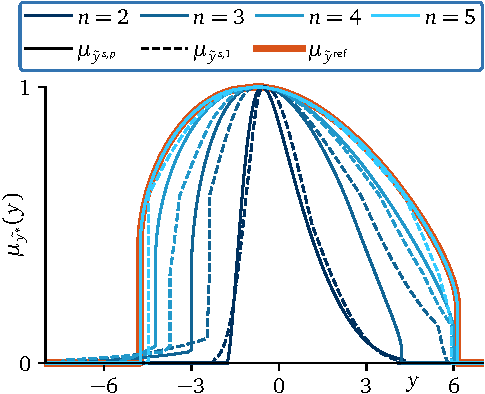
\includegraphics{resultsFuzzyPropagation_1}%
  \caption[Convergence of fuzzy output intervals]{%
    Convergence of the membership functions of the fuzzy output intervals
    $\fuzzy[\sparse,p]{y}$
    (\emph{solid lines,} modified hierarchical cubic not-a-knot B-splines)
    and $\fuzzy[\sparse,1]{y}$
    (\emph{dashed,} modified hierarchical hat functions)
    to the reference solution $\fuzzy[\reference]{y}$
    \emph{\textcolor{C1}{(red)}} for the bivariate Alp02 function using
    regular sparse grids of level $n = 2, \dotsc, 5$.%
  }%
  \label{fig:resultsFuzzyPropagation}%
\end{SCfigure}

In \cref{fig:resultsFuzzyRegular}, we study the convergence of the
relative $\Ltwo$ errors
\begin{equation}
  e^{\sparse,\ast}
  \ceq \frac{
    \normLtwo{\memfun[\reference]{y} - \memfun[\sparse,\ast]{y}}
  }{
    \normLtwo{\memfun[\reference]{y}}
  },\quad
  \ast \in \{1, p\},
\end{equation}
of the membership functions (``fuzzy errors'').
The Alp02 ($d = 2$) errors
that correspond to \cref{fig:resultsFuzzyPropagation}
are shown in green in the left-most plot of \cref{fig:resultsFuzzyRegular}.
For the Bra02, GoP\punctfix{,} and Alp02 functions,
B-spline surrogates achieve
dramatic improvements over the hat function surrogates in the bivariate case.
For the bivariate Ack function, B-splines yield an error that
is still an order of magnitude smaller than the error of hat functions.
Just little or even no improvement can be seen
for the functions Sch06 and Sch22 with discontinuous derivatives or
higher dimensionalities $d \ge 4$.

\begin{figure}
  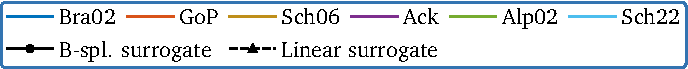
\includegraphics{resultsFuzzyLegend_1}\\[2mm]%
  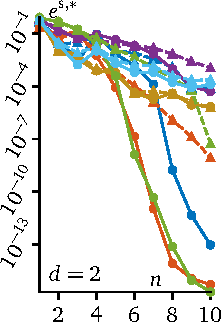
\includegraphics{resultsFuzzyRegular_1}%
  \hfill%
  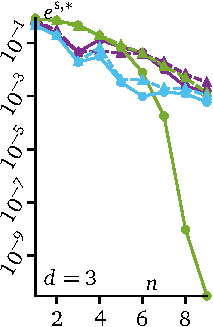
\includegraphics{resultsFuzzyRegular_2}%
  \hfill%
  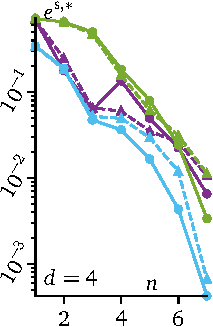
\includegraphics{resultsFuzzyRegular_3}%
  \hfill%
  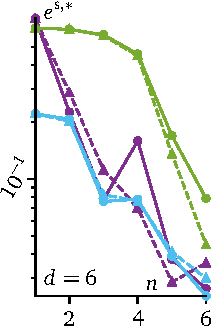
\includegraphics{resultsFuzzyRegular_4}%
  \caption[Fuzzy errors for regular sparse grids]{%
    Fuzzy errors
    $e^{\sparse,\ast}
    \ceq \normLtwo{\memfun[\reference]{y} - \memfun[\sparse,\ast]{y}}/
    \normLtwo{\memfun[\reference]{y}}$
    for regular sparse grids $\regsgset{n}{d}$
    and different objective functions $\objfun$ \emph{(colors)}
    over the level $n$ of the sparse grid.%
  }%
  \label{fig:resultsFuzzyRegular}%
\end{figure}

\paragraph{Fuzzy Novak--Ritter method}

We want to employ spatial adaptivity to improve the results
of regular sparse grids.
To this end, we modify the Novak--Ritter criterion
to create a grid generation method that is tailored for the
fuzzy extension principle, resulting in \cref{alg:fuzzyNovakRitterMethod}.
Its main idea is to generate more points near the optima
of the fuzzy extension principle
(\cref{alg:alternativeFuzzyExtensionPrinciple}) than in other regions
of $\clint{\*0, \*1}$.
Therefore, we apply the Novak--Ritter criterion twice to
every $\alpha$ level $\alpha_j = \tfrac{j}{m}$ ($j = 0, \dotsc, m$),
once for the minimum and once for the maximum.
For all $\alpha_j$, the points to be refined are collected in a set.
If a point is selected multiple times for different $\alpha_j$,
it is refined only once.
In addition, we enlarge the search domain $\Omega_{\alpha_j}$
by \SI{10}{\percent}, since the minimum or the maximum might be
near the boundary $\Omega_{\alpha_j}$ and
since the points to be inserted might not be close to
the points to be refined.
We ensure that the size of $\Omega_{\alpha_j}$ is at least $0.05$
in every coordinate direction.
The remaining experiments use $\gamma = 0.1$ as adaptivity.

\begin{algorithm}
  \begin{algorithmic}[1]
    \Function{$\liset = \texttt{fuzzyNovakRitterMethod}$}{%
      $\objfun$, $\gamma$, $m$, $\liset$, $\fuzzy{x}_1$, \dots, $\fuzzy{x}_d$%
    }
      \ForOneLine{$(\*l, \*i) \in \liset$}{$d_{\*l,\*i} \gets 0$}
      \Comment{degrees (number of refinements)}%
      \While{$\setsize{\liset} < \ngpMax$}
        \State{$R \gets \emptyset$}
        \For{$j = 0, \dotsc, m$}
          \State{$\alpha_j \gets j/m$}
          \For{$t = 1, \dotsc, d$}
            \State{$\clint{a_{j,t}, b_{j,t}} \gets \acut[t]{x}{\alpha_j}$}
            \Comment{determine $\alpha_j$-cut}%
            \If{$b_{j,t} - a_{j,t} < 0.05$}
            \Comment{ensure minimal size of $0.05$}%
              \State{%
                $(a_{j,t}, b_{j,t}) \gets
                ((a_{j,t} + b_{j,t})/2 - 0.025,
                (a_{j,t} + b_{j,t})/2 + 0.025)$%
              }\vspace{-1mm}
            \EndIf{}
            \State{%
              $(a_{j,t}, b_{j,t}) \gets
              (a_{j,t} - 0.05 (b_{j,t} - a_{j,t}),
              b_{j,t} + 0.05 (b_{j,t} - a_{j,t}))$%
            }
            \Comment{enlarge by \SI{10}{\percent}}%
            \vspace{-1mm}
          \EndFor{}
          \State{%
            $\liset_j \gets \{(\*l, \*i) \in \liset \mid
            \gp{\*l,\*i} \in \clint{\*a_j, \*b_j} \cap \clint{\*0, \*1}\}$%
          }
          \Comment{%
            set of feasible points
            ($\clint{\*a_j, \*b_j} = \Omega_{\alpha_j}$)%
          }%
          \ForOneLine{$(\*l, \*i) \in \liset_j$}{%
            $r_{\*l,\*i} \gets \setsize{
              \{(\*l', \*i') \in \liset_j \mid
              \objfun(\gp{\*l',\*i'}) \le \objfun(\gp{\*l,\*i})\}
            }$%
          }
          \Comment{ranks}%
          \State{%
            $(\*l^\ast, \*i^\ast) \gets
            \vecargmin_{(\*l,\*i) \in \liset_j} \bracket*{
              (r_{\*l,\*i} + 1)^\gamma
              (\normone{\*l} + d_{\*l,\*i} + 1)^{1 - \gamma}
            }$%
          }
          \Comment{for minimum}%
          \vspace{-0.7mm}
          \State{%
            $(\*l^{\ast\ast}, \*i^{\ast\ast}) \gets
            \vecargmin_{(\*l,\*i) \in \liset_j} \bracket*{
              (\setsize{\liset_j} - r_{\*l,\*i} + 2)^\gamma
              (\normone{\*l} + d_{\*l,\*i} + 1)^{1 - \gamma}
            }$%
          }
          \Comment{for maximum}%
          \State{%
            $R \gets R \cup \{(\*l^\ast, \*i^\ast),
            (\*l^{\ast\ast}, \*i^{\ast\ast})\}$%
          }
        \EndFor{}
        \State{Refine all points in $\liset$ that are in $R$}
        \ForOneLine{$(\*l, \*i) \in R$}{$d_{\*l,\*i} \gets d_{\*l,\*i} + 1$}
      \EndWhile{}
    \EndFunction{}
  \end{algorithmic}
  \caption[Fuzzy Novak--Ritter method]{%
    Fuzzy Novak--Ritter method to generate spatially adaptive sparse grids
    for the fuzzy extension principle.
    Inputs are
    the objective function $\objfun$,
    the adaptivity parameter $\gamma \in \clint{0, 1}$,
    the number of $\alpha$ segments,
    the initial sparse grid $\liset$ as a set of level-index pairs, and
    the $d$ fuzzy intervals $\fuzzy{x}_1, \dotsc, \fuzzy{x}_d$.
    The output is the spatially adaptive sparse grid $\liset$.%
  }%
  \label{alg:fuzzyNovakRitterMethod}%
\end{algorithm}

\paragraph{Convergence of fuzzy intervals on spatially adaptive sparse grids}

As we can see in \cref{fig:resultsFuzzyAdaptive},
the spatially adaptive sparse grids generated by the fuzzy Novak--Ritter
method improve results significantly
for both cubic B-spline and piecewise linear surrogates.
However, the performance of the B-spline surrogates benefits more
from the spatial adaptivity.
Even for higher-dimensional settings such as $d = 6$,
the spatial adaptivity helps to decrease the errors by one order of magnitude.
For instance, for the Ack function in six variables,
we can achieve an error of \SI{2.6}{\percent}
with a budget of \num{10000} objective function evaluations (grid points)
on regular sparse grids.
With the same budget and with spatial adaptivity, the error drops below
\SI{0.25}{\percent}.
Conversely, to achieve the same error as in the regular case
(\SI{2.6}{\percent}),
only \SI{1600} evaluations are needed for spatially adaptive grids.

\begin{figure}
  \includegraphics{resultsFuzzyLegend_2}\\[2mm]%
  \includegraphics{resultsFuzzyAdaptive_1}%
  \hfill%
  \includegraphics{resultsFuzzyAdaptive_2}%
  \hfill%
  \includegraphics{resultsFuzzyAdaptive_3}%
  \caption[Fuzzy errors for spatially adaptive sparse grids]{%
    Fuzzy errors
    $e^{\sparse,\ast}
    \ceq \normLtwo{\memfun[\reference]{y} - \memfun[\sparse,\ast]{y}}/
    \normLtwo{\memfun[\reference]{y}}$
    for spatially adaptive sparse grids $\sgset$ \emph{(solid markers)}
    and different objective functions $\objfun$ \emph{(colors)}
    over the number $\ngpMax$ of objective function evaluations.
    For comparison, the results of \cref{fig:resultsFuzzyRegular}
    for regular sparse grids are repeated \emph{(hollow markers).}%
  }%
  \label{fig:resultsFuzzyAdaptive}%
\end{figure}


\cleardoublepage
